\documentclass{config/apuntes}

\title{Análisis de secuencias}
\author{Sandra Mingo Ramírez}
\date{2024/25}
\acronym{SEQAN}

\usepackage[all]{nowidow}
\usepackage{listing}
\usepackage{color}
\usepackage{tabularx}
\usepackage{multirow}
\usepackage{makecell}
\usepackage{amsmath}
\usepackage{array}

\definecolor{dkgreen}{rgb}{0,0.6,0}
\definecolor{gray}{rgb}{0.5,0.5,0.5}
\definecolor{mauve}{rgb}{0.58,0,0.82}

\lstset{
  language=Python,
  frame=tb,
  aboveskip=3mm,
  belowskip=3mm,
  showstringspaces=false,
  columns=flexible,
  basicstyle={\small\ttfamily},
  numbers=none,
  numberstyle=\tiny\color{gray},
  keywordstyle=\color{blue},
  commentstyle=\color{dkgreen},
  stringstyle=\color{mauve},
  breaklines=true,
  breakatwhitespace=true,
  tabsize=3
}

\begin{document}

\begin{abstract}
El análisis de secuencias es una herramienta clave en bioinformática que permite descifrar la información contenida en las secuencias de ADN, ARN y proteínas. A través de modelos computacionales y estadísticos, es posible estudiar patrones, predecir funciones y entender la relación (evolutiva) entre secuencias y su impacto biológico. El objetivo de este curso es entender cómo y por qué analizamos secuencias biológicas, enfatizando en el fundamento algorítmico y biológico de estas herramientas. 
\end{abstract}

\pagestyle{plain}

\maketitle

\tableofcontents

%Hay apuntes de clase subidos a Perusall del profesor
%El día 28/10 es el último día y se escribirá el examen final. Otra opción es no ir ese día y presentarnos al examen de enero, pero no se podrá ir a ambos. En caso de suspender, la siguiente convocatoria es en junio. En el examen no habrá que codificar, pero sí podrá ponernos algún código y pedir cómo funciona o cómo lo aplicaríamos. 60% de la nota final. 
%La nota se divide en el examen final y una serie de entregas, entre las cuales se incluyen quizz, ejercicios de programación y un quiz final de autoevaluación. 40% de la nota final

%27/09 - Luis del Peso
\chapter{Modelos estadísticos en el análisis de secuencias}
\section{Secuencias biológicas como cadenas o strings}
El ADN, el ARN y las proteínas son responsables del almacenamiento, mantenimiento y ejecución de la información genética, representando así el dogma central de la biología molecular. Estas moléculas están compuestas por miles de átomos dispuestos en complejas estructuras tridimensionales. Y lo que es más importante, la estructura de estas moléculas es clave para su función. Una característica notable común a estas biomoléculas es que, a pesar de su complejidad estructural, son \textbf{polímeros lineales de un número limitado de subunidades (monómeros)} y un gran número de pruebas experimentales indican que la secuencia de los monómeros en la estructura lineal de estas moléculas es el principal determinante de sus propiedades, incluidas la estructura y la función. Así pues, estas moléculas pueden conceptualizarse como cadenas de símbolos y este sencillo modelo capta sus propiedades más fundamentales. Sorprendentemente, esta abstracción coincide con la definición formal de una cadena en las herramientas matemáticas y computacionales.

\subsection{Definición formal de una cadena}
En los lenguajes formales, como los utilizados en matemáticas e informática, una cadena se define como una secuencia finita de símbolos de un alfabeto determinado. Sea $\Sigma$ un conjunto finito no vacío de símbolos (caracteres), llamado alfabeto. Una cadena sobre $\Sigma$ es cualquier secuencia finita de símbolos de $\Sigma$. El número total de símbolos de una cadena s se conoce como longitud de secuencia, o simplemente longitud, y se suele representar como $||s||$. Una palabra suele ser una cadena sobre $\Sigma$ de longitud definida. El conjunto de todas las cadenas de longitud n sobre $\Sigma$, es decir, el conjunto de todas las palabras de tamaño n, se denomina $\Sigma^n$. Existen varias operaciones definidas para las cadenas, que también pueden representarse como nodos de un gráfico. En realidad, esto es clave para algunos métodos computacionales utilizados para ensamblar genomas completos a partir de estrategias de secuenciación shotgun.

\subsection{ADN como cadena}
Una molécula de ADN puede idealizarse como una cadena sobre el conjunto \{A, C, G, T\}, donde cada símbolo representa uno de los cuatro monómeros de nucleótidos del ADN, y una proteína como una cadena sobre el conjunto \{A, C, D, E, F, G, H, I, K, L, M, N, P, Q, R, S, T, V, W, Y\}, donde cada símbolo representa cada uno de los 20 residuos de aminoácidos (monómeros) presentes en las proteínas naturales. Si $\Sigma = \{A, C, G, T\}$, entonces $\Sigma^3$ representa los codones del código genético.

\section{Modelos estadísticos del ADN}
Consideremos que queremos construir un dispositivo (podría ser un programa informático o un artefacto físico como una ruleta, véase más adelante) que pueda producir una secuencia de ADN (es decir, una cadena sobre el conjunto \{A, C, G, T\}) que sea una cadena que tenga las mismas propiedades (composición y distribución de nucleótidos) que las moléculas de ADN reales. Para ello podemos utilizar dos modelos: el modelo multinomial y el modelo de cadena de Markov.

\subsection{Modelo multinomial}
El modelo más simple de secuencias de ADN asume que los nucleótidos son independientes e idénticamente distribuidos (iid), es decir, la secuencia ha sido generada por un proceso que produce cualquiera de los cuatro símbolos en cada posición de secuencia i al azar, extrayéndolos independientemente de la misma distribución de probabilidad \footnote{Una distribución de probabilidad es una lista de los posibles resultados con sus correspondientes probabilidades que cumple tres reglas: 1. los resultados deben ser disjuntos; 2. cada probabilidad debe estar comprendida entre 0 y 1; 3. las probabilidades deben sumar 1.} sobre el alfabeto \{A, C, G, T\}.

Se puede generar una secuencia de ADN según el modelo multinomial \footnote{La distribución binomial describe la probabilidad de obtener un número determinado de éxitos en n experimentos independientes. Fundamentalmente, la distribución binomial se aplica sólo cuando el experimento tiene sólo dos resultados posibles. La distribución multinomial es una generalización de la distribución binomial donde cada variable aleatoria puede tomar más de dos valores.} utilizando un dispositivo sencillo como el que se representa en la figura \ref{fig:ruletas}. El modelo de secuencia multinomial es como tener una ruleta que se divide en cuatro partes diferentes etiquetadas como A, T, G y C, donde pA, pT, pG y pC son las fracciones de la ruleta ocupadas por los cortes con estas cuatro etiquetas. Si se hace girar la flecha situada en el centro de la rueda de la ruleta, la probabilidad de que se detenga en la porción con una etiqueta particular (por ejemplo, la porción etiquetada como "A") solo depende de la fracción de la rueda ocupada por esa porción (pA aquí).

\begin{figure}[htbp]
\centering
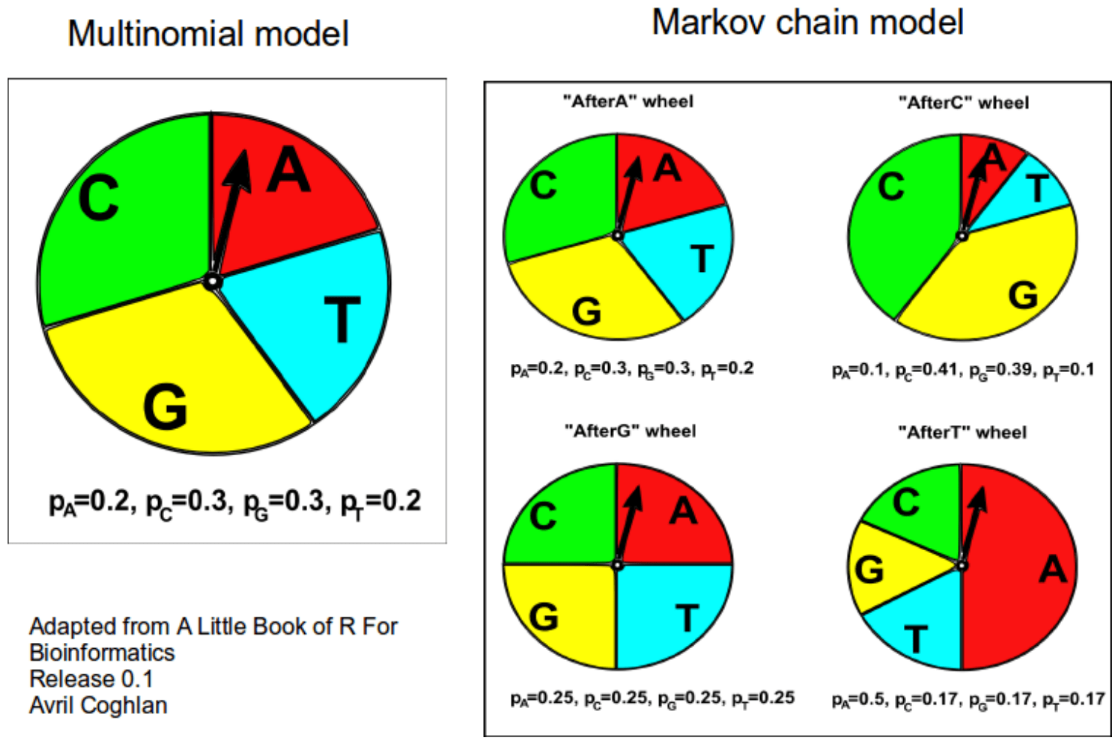
\includegraphics[width = 0.55\textwidth]{figs/ruletas.png}
\caption{Comparación de los modelos de secuencia de ADN multinomial y cadena de Markov. }
\label{fig:ruletas}
\end{figure}

En una cadena generada por un modelo multinomial, la probabilidad de observar el símbolo (nucleótido en el caso del ADN y aminoácido en el caso de la proteína) x en la posición i de la secuencia se denota por $p_x,i = p(s(i)=x)$ y no depende de la posición i. Por lo tanto, podemos calcular la probabilidad de observar la cadena s donde n = ||s|| como:

 $$ p(s) = \prod_{i=1}^{n} p(s_i) $$

\textit{Ejemplo práctico:}
En un experimento ChIP-seq (una técnica de secuenciación masiva que permite identificar sitios de unión de proteínas al ADN), se descubrieron 500 sitios de unión para un factor de transcripción. Dado que el genoma humano contiene entre 20,000 y 26,000 genes, estos 500 sitios pueden parecer pocos. Sin embargo, la cuestión central es si esta cantidad es coherente con lo que se esperaría bajo un modelo estadístico.
Los factores de transcripción se unen a subsecuencias específicas de ADN llamadas "motivos de respuesta". En este caso, el motivo de unión es RCGTG, donde R representa A o G. Aunque las moléculas biológicas interaccionan con cierta flexibilidad, este motivo es bastante restringido, ya que solo una posición es flexible. El genoma humano tiene alrededor de $3 \times 10^9$ bases, por lo que podemos calcular la cantidad esperada de sitios de unión basándonos en la probabilidad de que este motivo ocurra aleatoriamente.
Asumiendo que los nucleótidos son independientes entre sí y tienen la misma probabilidad de aparecer, la probabilidad de que aparezca la secuencia CGTG es $0,25^4$. Para la posición R, que puede ser A o G, la probabilidad es $0,5$. Por tanto, la probabilidad total de encontrar el motivo RCGTG es $0,25^4 \times 0,5 = \frac{1}{512}$, es decir, se esperaría encontrar esta secuencia una vez cada 512 posiciones. Con un genoma de $3 \times 10^9$ bases, se esperaría aproximadamente $\frac{3 \times 10^9}{512} \approx 6 \times 10^6$ sitios. Sin embargo, en el experimento solo se hallaron 500 sitios, lo que sugiere que el modelo experimental no refleja completamente la realidad biológica y es necesario recurrir a otros modelos, aunque sean simplificados.
La secuencia por sí sola no es suficiente para que el factor de transcripción se una. Otros factores, como la accesibilidad de la cromatina, también juegan un papel crucial. No obstante, el modelo multinomial proporciona una referencia útil para evaluar los datos experimentales en un contexto aleatorio.
Si bien este enfoque es sencillo, tiene limitaciones significativas, como la suposición de independencia entre nucleótidos. Sabemos que esto no es siempre cierto, por ejemplo, los dinucleótidos CG suelen ser menos frecuentes salvo en las "islas CpG", donde existe una gran concentración.

\subsubsection{Frecuencia de dinucleótidos}
Los dinucleótidos, que representan todas las combinaciones posibles de dos nucleótidos ($\Sigma^2$), deberían tener una frecuencia esperada de $\frac{1}{16}$ en el genoma humano. Al analizar las frecuencias observadas en el cromosoma 21, se encuentra que A y T aparecen con una frecuencia del 29.5\%, mientras que G y C con un 20.5\% (Figura \ref{fig:dinucleotidos}). Al recalcular las frecuencias de los dinucleótidos, se observa que, en general, la frecuencia observada coincide con la esperada, excepto para el dinucleótido CG, cuya frecuencia observada es tres veces menor a la esperada. Esto sugiere que los nucleótidos no son completamente independientes, y el modelo multinomial no es suficiente para describir esta dependencia.

\begin{figure}[htbp]
\centering
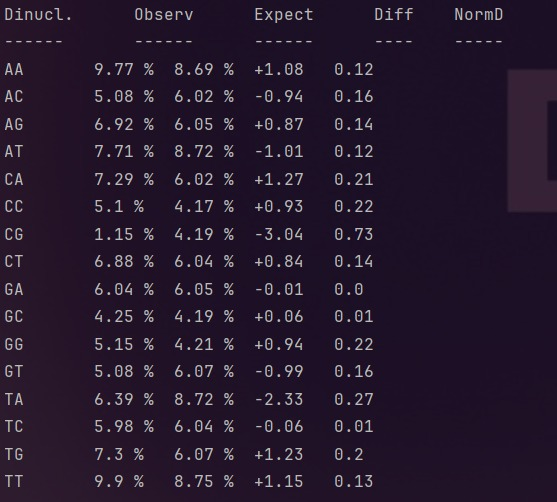
\includegraphics[width = 0.55\textwidth]{figs/freqs-dinucleotidos.jpg}
\caption{Cálculo de las frecuencias de los 16 dinucleótidos en el cromosoma 21 del ser humano. Los valores esperados y observados suelen coincidir en $\pm$ 1\% a excepción del dinucleótido CG. }
\label{fig:dinucleotidos}
\end{figure}
 
\subsection{Cadena de Markov}
El modelo multinomial es una herramienta sencilla e intuitiva que representa con precisión muchas secuencias biológicas de ADN. Sin embargo, se supone que la probabilidad de que aparezca un nucleótido en una posición determinada es independiente de la identidad de los residuos cercanos, lo que no siempre es así. Por ejemplo, si quisiéramos modelar un tramo de ADN que comprende una isla CpG, la probabilidad de observar una G estaría estrictamente condicionada a la identidad del residuo anterior, es decir, la probabilidad de observar una G después de una C sería probablemente más alta que después de cualquier otro residuo de nucleótido. Las cadenas de Markov pueden modelar correlaciones locales entre símbolos en una cadena. Para ello utilizan probabilidades condicionales. Por lo tanto, mientras que en el modelo multinomial se suponía que pG era constante a lo largo de la secuencia, en el modelo de cadena de Markov pG después de C $p(G|C)$ no es necesariamente igual a pG después de A $p(G|A)$.
Se puede generar una secuencia de ADN según el modelo de Markov utilizando un dispositivo sencillo como el que se muestra a la derecha en las figuras \ref{fig:ruletas} y \ref{fig:markov}. En este caso tenemos cuatro ruletas, cada una de las cuales representa las probabilidades de los nucleótidos del ADN. Para generar un residuo en cualquier posición determinada usando este modelo, elegiríamos una de estas cuatro ruedas de ruleta dependiendo del residuo que obtuviéramos en la posición anterior. Se podría representar todas estas probabilidades usando una matriz donde las filas representan el nucleótido encontrado en la posición anterior de la secuencia, mientras que las columnas representan los nucleótidos que podrían encontrarse en la posición actual de la secuencia. En la tabla \ref{tab:matrix} se muestra una representación de la ruleta a la derecha de la figura \ref{fig:ruletas} en forma de matriz.

\begin{table}[htbp]
    \centering
    \begin{tabularx}{\textwidth}{ X | X X X X}
          & To A & To C & To G & To T \\ \hline
         From A & 0,20 & 0,30 & 0,30 & 0,20 \\
         From C & 0,10 & 0,41 & 0,39 & 0,10 \\
         From G & 0,25 & 0,25 & 0,25 & 0,25 \\
         From T & 0,50 & 0,17 & 0,17 & 0,17 \\
    \end{tabularx}
    \caption{Matriz de transición de cadena de Markov.}
    \label{tab:matrix}
\end{table}

En la jerga de los modelos de Markov, esta matriz se denomina \textbf{matriz de transición}. La razón es que una cadena de Markov generadora de secuencia de ADN se puede idealizar como una estructura con cuatro estados diferentes, que representan cada uno de los cuatro nucleótidos, y la secuencia se produce por la transición de un estado a otro. Las transiciones entre estados no son igualmente probables, sino que ocurren con las probabilidades indicadas en los bordes que unen cada estado, que en conjunto son las probabilidades de transición y pueden representarse como una matriz de transición (véase figura \ref{fig:markov}).
Las entradas en la matriz de transición corresponden a probabilidades condicionales. Por ejemplo, pCG es la probabilidad de G en la posición i dado que hay una C en la posición i-1, es decir $pG = p(s_i = G|s_{i-1} = C)$. Por tanto, la probabilidad de la secuencia s según este modelo podría calcularse como $ p(s) = \prod p(s_i | s_{i-1}) $. Sin embargo, vale la pena señalar que, para representar una molécula de ADN lineal, también necesitaríamos un conjunto de parámetros que representen las probabilidades del primer nucleótido en la secuencia (dado que no hay uno anterior, podríamos obtener esta probabilidad de la matriz de transición). Si definimos estas probabilidades iniciales como $\pi(A), \pi(C), \pi(G), \pi(T)$, entonces la probabilidad de una secuencia lineal según este modelo se puede calcular como:

 $$ p(s) = \pi(s_1) * \prod_{i=2}^{n} p(s_i | s_{i-1}) $$
 
\begin{figure}[htbp]
\centering
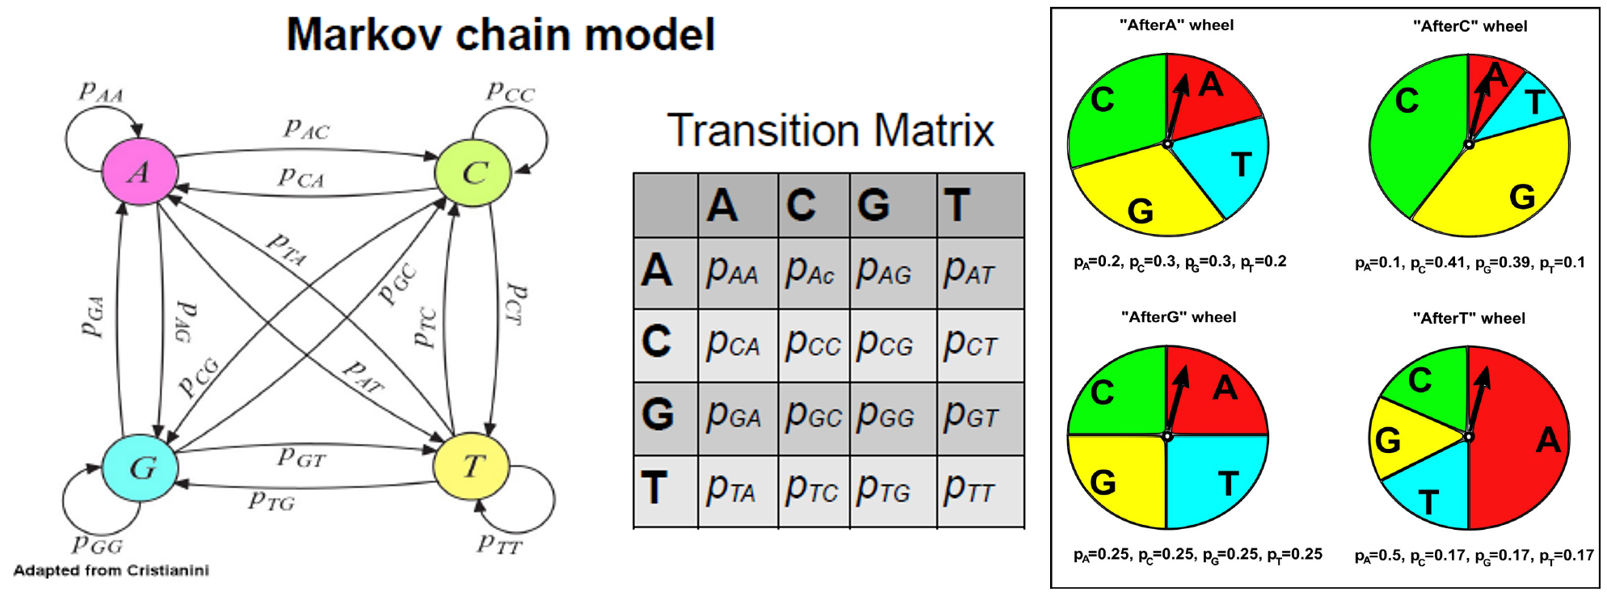
\includegraphics[width = 0.7\textwidth]{figs/markov.png}
\caption{Representaciones gráficas de la cadena de Markov. En la matriz de transición, las filas corresponden a los nucleótidos de la posición anterior y las columnas los nucleótidos que les siguen. }
\label{fig:markov}
\end{figure}
 
Por ejemplo, para calcular la probabilidad de encontrar la secuencia RCGTG utilizando este modelo, se deben considerar las probabilidades condicionales para cada posible combinación de nucleótidos. La probabilidad se calcula dividiendo la secuencia en dos casos, que luego se suman:
\begin{align*}
0,25 \times 0,3 \times 0,39 \times 0,25 \times 0,17 (ACGTG) \\
+ 0,25 \times 0,25 \times 0,39 \times 0,25 \times 0,17 (GCGTG) \\
= 0,001243 + 0,001036 \\
= 0,002279 
\end{align*}
 
\subsection{Ejercicios}
\textit{\textbf{Ejercicio 1:} 
Supongamos que el ADN humano puede dividirse en sólo dos tipos de regiones las ricas en C+G y el resto del ADN con una composición de bases no sesgada (no ricas en C+G). Suponiendo el modelo de independencia (la probabilidad de cada nucleótido en una posición dada es independiente de la identidad de los nucleótidos adyacentes) y que la secuencia es homogénea dentro de cada una de estas dos regiones, podemos representarlas mediante un modelo probabilístico multinomial. La región rica en G+C se define por los parámetros: pT=1/8, pC=3/8,pA=1/8 y pG=3/8. El resto del ADN por pT=pC=pA=pG=1/4. ¿Cuál es la probabilidad de observar la secuencia seg=CGACGCGCGCGTCG en una región rica en C+G? ¿Y en la no rica en G+C? Ahora bien, imaginemos que sólo el 1\% (¡me lo acabo de inventar!) del genoma es rico en C+G. Si tomamos un genoma de 14 pb al azar y resulta ser la secuencia CGACGCGCGCGTCG, ¿cuál sería la probabilidad de que proceda de una región rica en C+G?}
\begin{itemize}
\item Paso 1: Probabilidad de observar la secuencia en la región rica en C+G

La probabilidad de observar una secuencia en una región rica en C+G, dada la independencia entre los nucleótidos, es el producto de las probabilidades de cada nucleótido en la secuencia. Las probabilidades en la región rica en C+G son las siguientes:

\[
p_T = \frac{1}{8}, \quad p_C = \frac{3}{8}, \quad p_A = \frac{1}{8}, \quad p_G = \frac{3}{8}
\]

Dada la secuencia \texttt{CGACGCGCGCGTCG}, la probabilidad de observarla en la región rica en C+G es:

\[
P(\text{CGACGCGCGCGTCG} \mid \text{C+G}) = p_C \cdot p_G \cdot p_A \cdot p_C \cdot p_G \cdot p_C \cdot p_G \cdot p_C \cdot p_G \cdot p_C \cdot p_G \cdot p_T \cdot p_C \cdot p_G
\]

Sustituyendo los valores de las probabilidades:

\small
\[
P(\text{CGACGCGCGCGTCG} \mid \text{C+G}) = 
\]

\[
\left( \frac{3}{8} \right) \cdot \left( \frac{3}{8} \right) \cdot \left( \frac{1}{8} \right) \cdot \left( \frac{3}{8} \right) \cdot \left( \frac{3}{8} \right) \cdot \left( \frac{3}{8} \right) \cdot \left( \frac{3}{8} \right) \cdot \left( \frac{3}{8} \right) \cdot \left( \frac{3}{8} \right) \cdot \left( \frac{3}{8} \right) \cdot \left( \frac{3}{8} \right) \cdot \left( \frac{1}{8} \right) \cdot \left( \frac{3}{8} \right) \cdot \left( \frac{3}{8} \right)
\]

\normalsize

\item Paso 2: Probabilidad de observar la secuencia en la región no rica en C+G

En la región no rica en C+G, las probabilidades de cada nucleótido son iguales:

\[
p_T = p_C = p_A = p_G = \frac{1}{4}
\]

Por lo tanto, la probabilidad de observar la secuencia \texttt{CGACGCGCGCGTCG} es:

\[
P(\text{CGACGCGCGCGTCG} \mid \text{no C+G}) = \left( \frac{1}{4} \right)^{14}
\]

\item Paso 3: Probabilidad de que la secuencia provenga de una región rica en C+G

Utilizamos el teorema de Bayes para calcular la probabilidad de que la secuencia provenga de una región rica en C+G. La fórmula de Bayes es:

\[
P(\text{C+G} \mid \text{secuencia}) = \frac{P(\text{secuencia} \mid \text{C+G}) \cdot P(\text{C+G})}{P(\text{secuencia})}
\]

Donde:
\begin{itemize}
\item $ P(\text{secuencia} \mid \text{C+G}) $ es la probabilidad de observar la secuencia en una región rica en C+G (calculada en el Paso 1).
\item $ P(\text{C+G}) = 0{.}01 $ es la proporción del genoma que es rico en C+G.
\item $ P(\text{secuencia}) $ es la probabilidad total de observar la secuencia, que se calcula como:
\end{itemize}

\[
P(\text{secuencia}) = P(\text{secuencia} \mid \text{C+G}) \cdot P(\text{C+G}) + P(\text{secuencia} \mid \text{no C+G}) \cdot P(\text{no C+G})
\]

Donde $ P(\text{no C+G}) = 1 - P(\text{C+G}) = 0{.}99 $

Sustituyendo todos los valores, podemos obtener la probabilidad de que la secuencia provenga de una región rica en C+G.
\end{itemize}

\textit{\textbf{Ejercicio 2:} 
Ha secuenciado un fragmento de la cadena + de un nuevo organismo. Nosotros suponemos que es un fragmento representativo y que la composición es homogénea en todo el genoma. Las frecuencias absolutas de bases en este fragmento de secuencia se indican en la tabla siguiente. Estima los siguientes parámetros de un modelo de cadena de Markov para esta secuencia. ¿Qué sería la probabilidad de transición de T a A (PTA) y la probabilidad de y la probabilidad de transición de A a A (PAA)? ¿Cuál sería la probabilidad PTA para el modelo de cadena de Markov de la cadena - de este dsADN? ¿Y la probabilidad de transición de transición PAA de la cadena -?}
\begin{table}[htbp]
    \centering
    \begin{tabularx}{\textwidth}{ X | X X X X}
          & To A & To C & To G & To T \\ \hline
         From A & 15 & 23 & 25 & 11 \\
         From C & 9 & 38 & 35 & 8 \\
         From G & 26 & 21 & 18 & 24 \\
         From T & 25 & 8 & 10 & 3 \\
    \end{tabularx}
\end{table}
Teniendo en cuenta las siguientes probabilidades condicionales:
$$P_{TA+} = \frac{25}{25 + 8 + 10 + 3}$$
$$P_{AA+} = \frac{15}{15 + 23 + 25 + 11} $$

En cuanto a la probabilidad de la cadena negativa, hay que tener en cuenta que las frecuencias están dadas en la cadena positiva. Por tanto, cuando se tiene en cuenta el cambio del segundo nucleótido de la pareja en la cadena negativa, el cambio en la cadena positiva se produce en el primero. \\

\begin{table}[htbp]
\centering
5' -----------TA-----------3' \\
3' -----------AT-----------5' \\
\end{table}

$$P_{TA-} = \frac{25}{25 + 15 + 26 + 9}$$

\subsection{Problema práctico: islas CpG}
Un desafío interesante sería escribir un programa que identifique islas CpG en un fragmento del genoma humano. Los dinucleótidos CG tienden a perderse debido a la metilación de la citosina, que, al desaminarse, se convierte en timina en lugar de regresar a citosina. Sin embargo, en regiones del genoma que no se metilan, como las regiones transcripcionalmente activas, las secuencias CG permanecen intactas, formando las llamadas islas CpG. El objetivo del programa sería localizar el inicio y el final de una de estas islas en una secuencia genómica. La isla CpG tiene una longitud de 1.000 bases, mientras que la región genómica tendrá aproximadamente unos 40.000 nucleótidos.

\begin{figure}[htbp]
\centering
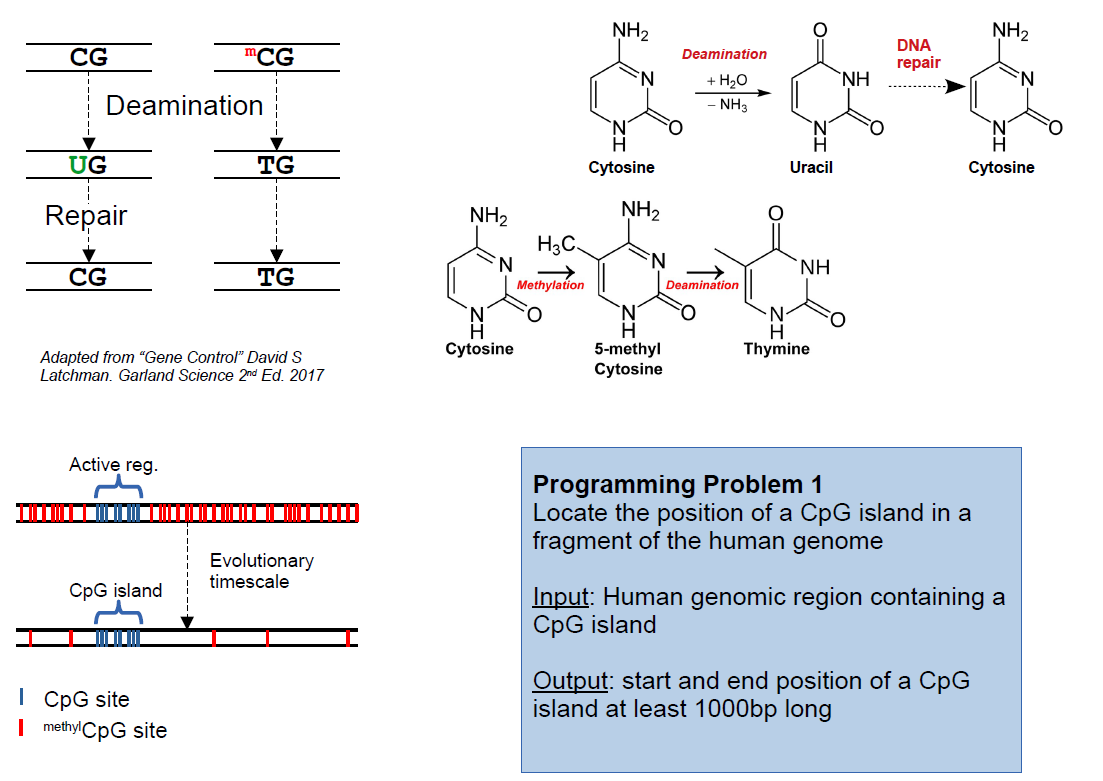
\includegraphics[width = 0.7\textwidth]{figs/cpg-islands.png}
\caption{Explicación biológica gráfica de las islas CpG. }
\end{figure}

Las islas CpG tienen una alta densidad de dinucleótidos de CG. Por tanto, hay que buscar una región genómica que tenga una alta densidad y que permita identificar la isla. Para ello, se debe emplear un sliding window, es decir, una ventana de una cierta cantidad de nucleótidos para calcular su frecuencia de CG. Como la isla CpG va a tener un tamaño de 1000, el tamaño razonable de ventana sería de 1000, y esta ventana se irá desplazando de nucleótido en nucleótido. En un gráfico que muestre la densidad de CG, se observaría una frecuencia muy superior (un pico alto) donde se encuentre la isla. Como la gráfica real es algo ruidosa, hay que establecer un threshold para poder obtener la posición concreta de la isla. Se puede utilizar la frecuencia total de CG en la secuencia (contabilizar todas las apariciones de CG y dividir por la longitud para obtener la media), pero hay que tener en cuenta el margen de error. Se puede calcular el porcentaje de CG en todas las ventanas, calcular la media y la desviación estándar para poder tener la dispersión esperada de una ventana concreta. Una vez con eso, se puede dibujar la distribución de los porcentajes de CpG para poder establecer la frecuencia de fondo de los dinucleótidos y separarla de la frecuencia de las islas CpG. En caso de una distribución normal, se pueden establecer criterios arbitrarios como los criterios estadísticos del 5\% superior (one value t-test). Esto resulta en una distribución empírica, pero se puede utilizar una distribución binomial para obtener el mismo resultado más formalmente correcto. También se puede aproximar a una distribución de Poisson para cada ventana. La forma más correcta sería mediante los modelos ocultos de Markov, teniendo como etiquetas que una posición pertenezca o no a una isla CpG. Esto se verá más adelante en la asignatura. 

%02/10 - Luis del Peso
\chapter{Alineamiento de secuencias por pares}
El alineamiento de secuencias es la herramienta más fundamental de la bioinformática. Permite identificar secuencias relacionadas con una secuencia dada. Como veremos, el parentesco suele implicar que las secuencias pueden tener funciones comunes y esa es una de las principales aplicaciones del alineamiento de secuencias, inferir la función de una secuencia biológica.

\section{Alineamiento de secuencias}
La alineación de secuencias es el procedimiento de ordenar dos (alineación por pares) o varias (alineación de secuencias múltiples, MSA) secuencias intentando colocar el mayor número posible de residuos idénticos o similares en el mismo registro vertical (misma columna). Los residuos no idénticos pueden colocarse en la misma columna como una falta de coincidencia o frente a un hueco en la otra secuencia. El objetivo de la alineación es maximizar el número de coincidencias (residuos idénticos o similares en la misma columna) y minimizar el número de desajustes y huecos.

\begin{figure}[htbp]
\centering
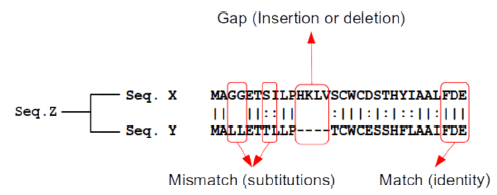
\includegraphics[width = 0.7\textwidth]{figs/pairwise-alignment.png}
\caption{\textbf{Alineamiento por pares.} La alineación por pares modela la evolución de las dos secuencias a partir de un ancestro común. En un intento de colocar los residuos derivados de la misma posición ancestral en el registro vertical, el proceso de alienación maximiza las coincidencias y minimiza las diferencias debidas a mutación de la secuencia ancestral (desajustes y lagunas). En la representación, dos residuos iguales se muestran conectados por una línea vertical. En caso de discordancia, si a nivel biológico los residuos tienen una función similar, se denota con dos puntos, mientras que si la función es diferente, se deja en blanco, al igual que en el caso de inserciones y deleciones.}
\end{figure}

¿Por qué alineamos las secuencias de este modo? En la alineación de secuencias, el supuesto subyacente es que las \textbf{secuencias que se alinean proceden de un ancestro común}. Sin embargo, como consecuencia de las mutaciones acumuladas durante la evolución, las secuencias no serán idénticas. Así pues, el reto consiste en colocar los residuos que derivan de la \textbf{misma posición ancestral} en la misma columna del alineamiento. Sin embargo, sin información sobre la secuencia ancestral y su evolución, lo mejor que podemos hacer es maximizar el número de coincidencias y minimizar el número de discordancias. En las secuencias de proteínas, las sustituciones se producen cuando una mutación (mutación sin sentido o missense) en la secuencia ancestral hace que el codón de un aminoácido se cambie por el de otro. El resultado sería la alineación de dos aminoácidos no idénticos, es decir, un desajuste. Las inserciones y deleciones (normalmente abreviadas como INDEL) se producen cuando se añaden o eliminan residuos de la secuencia ancestral. Las inserciones o deleciones (incluso las de un solo carácter) se representan como huecos en el alineamiento. El número de mutaciones aumentará a medida que las dos secuencias diverjan de su ancestro común. Así, en general, el número de coincidencias disminuye con la distancia evolutiva. En general, se puede inferir que los residuos idénticos entre secuencias probablemente también estén presentes en el ancestro. En el caso de las sustituciones y deleciones/inserciones, no se puede determinar si el ancestro era de una forma u otra, es decir, si realmente se trata de un fragmento que se ha perdido (una deleción) o un fragmento que en algún momento se insertó. 

\section{Comparación de alineamientos}
A la hora de alinear dos secuencias, se pueden producir todos los alineamientos posibles y escoger aquel que tenga el mayor número de coincidencias y el menor número de discordancias o gaps. Un alineamiento óptimo sería aquel que incluya en la misma columna residuos que derivan del mismo residuo original (es decir, alinear residuos ortólogos). Normalmente, no se conoce la secuencia del ancestro o la historia evolutiva, por lo que se intenta inferir al alinear todos los residuos idénticos o similares posibles. Para establecer el grado de similitud, se puede tener en cuenta las propiedades fisicoquímicas (hidrofobicidad, carga neta a pH fisiológico, flexibilidad de la cadena lateral) y la estructura (tamaño, presencia de anillos aromáticos). Además, si se permiten los gaps en el alineamiento, la cantidad de posibles alineamientos aumenta de forma astronómica. Por tanto, para encontrar el mejor alineamiento, se necesita:
\begin{itemize}
\item Una métrica cuantitativa que representa la similitud entre residuos.
\item Un método de puntuación que produce un valor que resume lo buena que es la alineación teniendo en cuenta todas las posiciones y huecos.
\item Un procedimiento capaz de producir todos los alineamientos posibles y puntuarlos eficazmente (y no evaluando todos los posibles alineamientos).
\end{itemize}

\subsection{Matrices de sustitución}
Como ya se ha dicho, el alineamiento consiste en reunir residuos idénticos o similares. Identificar los residuos idénticos es sencillo. Sin embargo, ¿qué entendemos por residuos similares? En el caso de los ácidos nucleicos, la función de un determinado nucleótido (su patrón de emparejamiento de bases) no suele poder sustituirse por ninguno de los demás nucleótidos. Por lo tanto, durante la alineación de secuencias de nucleótidos (normalmente) sólo nos preocupamos por las identidades \footnote{De hecho, dado que las transiciones (es decir, las sustituciones entre las purinas A y G o entre las pirimidinas C y T) son más frecuentes que las transversiones (sustituciones entre purina y pirimidina o viceversa), existen algunos esquemas de puntuación específicos para la alineación de residuos de nucleótidos no idénticos.}. Cualquier otro emparejamiento es un desajuste igualmente perjudicial. Sin embargo, en el caso de las secuencias de aminoácidos, ciertas sustituciones de aminoácidos tienen poco impacto, mientras que otras pueden abolir por completo la función/estructura de la proteína. Así, en el curso de la evolución, los residuos importantes para la función de la molécula tienden a permanecer inalterados o a ser sustituidos por un residuo similar, manteniendo así la estructura y/o la función. Por estas razones, algunas sustituciones particulares se encuentran comúnmente en proteínas relacionadas de diferentes especies. Así, para los alineamientos de proteínas asignamos una puntuación a cada par o aminoácidos que representa la probabilidad de observar la sustitución de uno por otro. Una tabla que contiene las puntuaciones de todos los posibles pares de residuos se denomina \textbf{matriz de sustitución}. Las puntuaciones de cada celda de una matriz de sustitución reflejan la probabilidad de que los dos residuos estén alineados porque son verdaderos homólogos en comparación con la probabilidad de que estén alineados en la misma posición por azar:

$$\frac{p(alineado|homologo)}{p(alineado|aleatorio)}$$

Estas probabilidades pueden derivarse de \textbf{principios teóricos}, por ejemplo el número de mutaciones necesarias para convertir el codón de un aminoácido en el de otro o la similitud fisicoquímica entre los dos residuos comparados. Sin embargo, las puntuaciones de las matrices de sustitución más populares se han derivado de la \textbf{observación empírica} de las tasas de sustitución en alineaciones de proteínas homólogas. Dos matrices de sustitución populares derivadas empíricamente son PAM y BLOSUM.

\subsubsection{Matrices de sustitución PAM}
Para construir una matriz de sustitución a partir de la observación de los reemplazos ocurridos durante la evolución, sólo necesitamos alinear las proteínas y contar el número de cambios de cada tipo. Sin embargo, generar una matriz de sustituciones a partir de alineamientos de proteínas es un problema circular: se necesita el alineamiento para contar el número de sustituciones observadas pero, para generar un buen alineamiento, se necesitan las puntuaciones de cada par de residuos. Para sortear este problema, Margaret Dayhoff (la primera bioinformática en la historia) y su equipo idearon una estrategia inteligente. Utilizaron secuencias muy similares de homólogos bien conocidos para poder generar alineaciones fácilmente y con gran confianza incluso en ausencia de matrices de sustitución. A continuación, a partir de estos alineamientos generaron árboles filogenéticos que les permitieron inferir la secuencia ancestral de cada par de proteínas alineadas. Por último, a partir de estos árboles calcularon las probabilidades de que cualquier aminoácido mutara en cualquier otro. Así, Dayhoff y sus colegas construyeron árboles filogenéticos a partir de familias de proteínas estrechamente relacionadas y calcularon la probabilidad de que dos residuos alineados derivaran del mismo residuo ancestral (véase la figura \ref{fig:pam}). En este proceso definieron una \textbf{mutación puntual aceptada} (abreviada como PAM) como la sustitución de un residuo original por otro que ha sido aceptado por la selección natural (de lo contrario no estaríamos observando estas secuencias). Como ya se ha mencionado, el conjunto original de proteínas que utilizaron para derivar la matriz de sustitución era muy similar y tenía 1 mutación puntual aceptada por cada 100 residuos de aminoácidos. En consecuencia, esta matriz se denomina PAM1.

Sin embargo, por definición, esta matriz es óptima para puntuar secuencias estrechamente relacionadas, pero no secuencias distantes (está sesgada a secuencias muy próximas evolutivamente). Para generar matrices que reflejaran relaciones más distantes, Dayhoff y sus colegas extrapolaron sus datos observados multiplicando PAM1 por sí mismo varias veces. Cuanto mayor era el número de veces que se multiplicaba el PAM1 por sí mismo, mayor era la distancia que representaba. Por ejemplo, PAM250, derivado de multiplicar PAM1 por sí mismo 250 veces, se utiliza habitualmente para comparar proteínas distantemente relacionadas.

\begin{figure}[htbp]
\centering
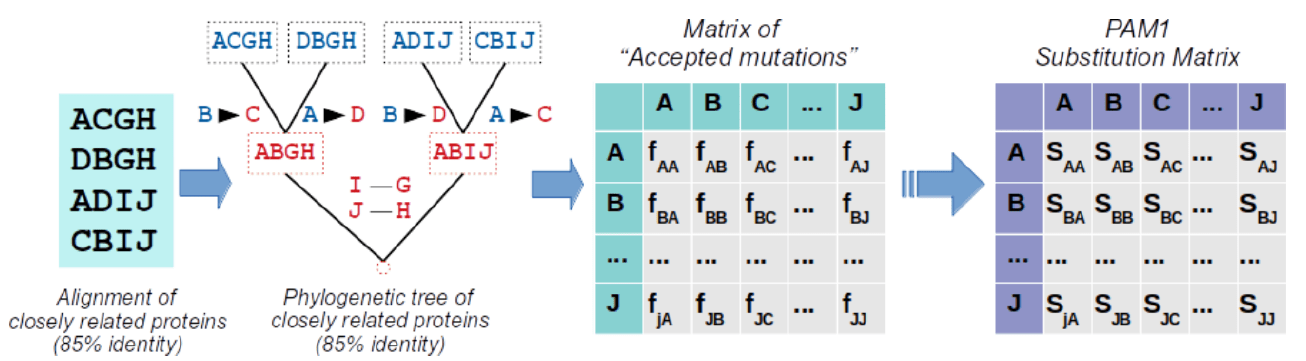
\includegraphics[width = \textwidth]{figs/pam-matrix.png}
\caption{\textbf{Generación de la matriz de sustitución PAM1.} A partir de alineaciones de secuencias estrechamente relacionadas (> 85\% de identidad), Margaret Dayhoff y sus colegas derivaron el árbol filogénico que representaba la evolución de la familia que requería el menor número de mutaciones. A partir de estos árboles contaron el número de veces que cada residuo fue sustituido por cualquier otro y registraron los valores en la matriz de mutaciones aceptadas. Por último, a partir de los datos de esta matriz generaron la matriz de sustitución PAM1 que representa la relación entre la probabilidad de la sustitución observada en el modelo evolutivo (suponiendo homología) y la probabilidad en el modelo aleatorio.}
\label{fig:pam}
\end{figure}

%04/10 - Luis del Peso
\subsubsection{Matrices de sustitución BLOSUM}
Más recientemente, el matrimonio Henikoff utilizó una familia de proteínas más alejada para poder inferir la frecuencia de sustitución en una matriz BLOSUM.

Para evitar la incertidumbre en los alineamientos, Dayhoff utilizó un conjunto de secuencias extremadamente relacionadas para derivar la PAM1. Sin embargo, las matrices PAM para proteínas más distantes se extrapolaron a partir de PAM1 en lugar de derivarse de la observación directa de los alineamientos reales. La acumulación de secuencias de proteínas en bases de datos a lo largo de los años permitió a Henikoff y Henikoff desarrollar un nuevo conjunto de matrices de sustitución a principios de los 90. Estas matrices, denominadas BLOCKS \footnote{un BLOCK se define como una región no superpuesta en el alineamiento de secuencias múltiples de menos de sesenta residuos de aminoácidos} amino acid SUbstitution Matrices (BLOSUM), se generaron al registrar cada posible sustitución de aminoácidos observada en los alineamientos de bloques. Utilizando alineamientos de proteínas que mostraban diferentes porcentajes de identidad, derivaron matrices BLOSUM que representaban la tasa de sustitución observada para diferentes grados de divergencia (figura \ref{fig:blosum}). Para ello, eliminan del bloque todas las secuencias que son idénticas en más de un x\% de posiciones, dejando una única secuencia representativa (por ejemplo, en BLOSUM62 se eliminaron las secuencias que compartían un 62\% de identidad o más). 

\begin{figure}[htbp]
\centering
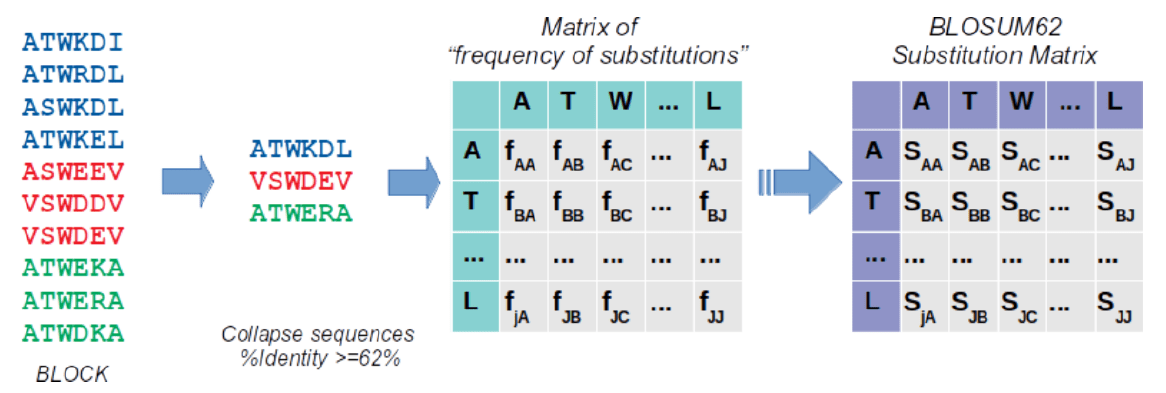
\includegraphics[width = \textwidth]{figs/blosum-matrix.png}
\caption{\textbf{Generación de la matriz de sustitución BLOSUM.} Partiendo de alineaciones sin colapsar de familias de proteínas (BLOCKS), Henikoff y Henikoff derivaron alineaciones que representaban diferentes distancias evolutivas colapsando todas las secuencias del bloque que compartían un umbral, C, de identidad. En la figura C = 62\%, todas las secuencias que comparten un porcentaje de identidad igual o superior al 62\% se muestran en el mismo color de fuente (primera columna), y luego se colapsan en un consenso que representa el clúster (segunda columna). A partir de estos alineamientos, contaron el número de veces que cada residuo i fue sustituido por cualquier otro y registraron los valores en la matriz de frecuencia de sustituciones. Por último, a partir de los datos de esta matriz generaron la matriz de sustituciones BLOSUM62 que representa la relación entre la probabilidad de la sustitución observada en el modelo evolutivo (suponiendo homología) y la probabilidad en el modelo aleatorio.}
\label{fig:blosum}
\end{figure}

Nótese que existen algunas diferencias importantes entre las matrices PAM y BLOSUM. En primer lugar, todas las matrices BLOSUM se derivan de la observación directa de alineamientos, mientras que sólo PAM se deriva de datos y el resto son extrapolaciones. En segundo lugar, mientras que PAM1 se generó a partir de alineaciones de secuencias estrechamente relacionadas (85\% de identidad), las matrices BLOSUM derivan de alineaciones que (pueden) incluir secuencias con un bajo porcentaje de identidad. Por último, para la construcción de PAM se infirieron sustituciones a partir de árboles filogenéticos derivados de los alineamientos. En BLOSUM no se construyó ningún árbol filogenético y las sustituciones se contaron a partir de la observación directa de los residuos alineados. Sin embargo, no se trata de sustituciones reales porque las secuencias alineadas evolucionaron a partir de un ancestro común y entre sí.

\subsubsection{Construcción de matrices de sustitución}
En las secciones anteriores vimos dos estrategias diferentes para determinar la frecuencia de cambios a partir de la observación empírica de alineamientos de proteínas homólogas. Dejando a un lado los detalles, ambos métodos producen una \textbf{matriz de frecuencia de mutación} \footnote{la suma de todas las entradas de la matriz da 1}, donde las entradas $q_{a,b}$, representan la \textbf{probabilidad observada} de encontrar los residuos a y b \textbf{alineados en proteínas homólogas}. En otras palabras, $q_{a,b}$, corresponde al término $p(alineado|homologo)$. Ahora, para obtener el valor de la entrada para los residuos a y b en la matriz de sustitución correspondiente, necesitamos calcular el término $p(alineado|aleatorio)$, que sería la \textbf{probabilidad esperada}. En el modelo aleatorio suponemos que las dos proteínas alineadas no están relacionadas y no existen restricciones estructurales o funcionales que puedan causar correlación entre los residuos en una posición dada. Así, en este modelo la probabilidad de encontrar los residuos a y b alineados sólo depende de su frecuencia en las proteínas. En el modelo aleatorio no existe correlación alguna entre los residuos alineados en una posición dada, por lo que la probabilidad de observar a en una secuencia y b en la otra son independientes de modo que:

$$p(alineado|aleatorio) = p(a \cap b) = p_a p_b $$

donde $p_a$, y $p_b$, son las frecuencias de a y b respectivamente. La probabilidad de observar a y b alineados en estos dos modelos puede compararse tomando el cociente de las probabilidades, denominado \textbf{odds ratio}: $q_{a,b}/(p_a p_b)$. Cuando la probabilidad en el modelo evolutivo es mayor que en el modelo aleatorio, el odds-ratio toma cualquier valor entre 1 e infinito. Sin embargo, cuando la probabilidad en el modelo aleatorio es mayor, la odds-ratio está entre 0 y 1. Para evitar esta asimetría, se suele tomar el logaritmo de la odds-ratio para obtener la \textbf{log-odds ratio}. Como veremos más adelante, tomar el logaritmo del odds-ratio también facilita el cálculo de la puntuación total de la alineación. Por lo tanto, la entrada en la matriz de sustitución correspondiente a a y b se calcula como:

$$ s_{a, b} = log \frac{q_{a, b}}{p_a p_b} = log \frac{p(cambio|modelo evolutivo)}{p(cambio|aleatorio)} = log \frac{p(observado)}{p(esperado)} $$

La figura \ref{fig:substitution} muestra las matrices de sustitución PAM250 y BLOSUM62. Dado que la puntuación del alineamiento a sobre b es la misma de b sobre a, estas matrices son simétricas. Por este motivo, normalmente sólo se representa la mitad de la matriz. Los números positivos significan que se han observado más veces el cambio de residuos que lo que cabría esperar por azar, por lo que debe haber alguna presión positiva para que se mantenga. En el caso de los números negativos, se debe a una selección negativa. Cuando es 0, el ratio es 1 y por tanto la frecuencia es la observada por azar, no hay ninguna presión. 

Un ejemplo: El triptófano tiene una frecuencia de mutación observada muy pequeña, pero en la tabla BLOSUM, su número es el más alto. Esto significa que es un aminoácido muy importante que no se puede cambiar por ningún otro. Así, la tabla de frecuencias per se no refleja el parecido entre residuos, ya que hay que tener en cuenta la frecuencia. Sin embargo, la tabla BLOSUM sí refleja el parecido entre los residuos.   

\begin{figure}[htbp]
\centering
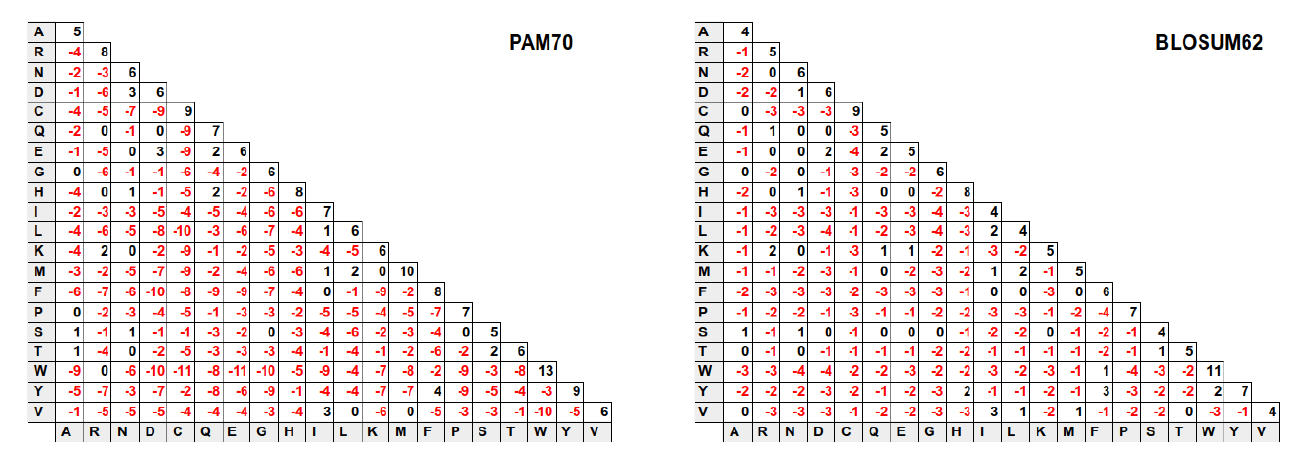
\includegraphics[width = \textwidth]{figs/substitution-matrix.png}
\caption{\textbf{Matrices de sustitución de aminoácidos.} La figura muestra las matrices de sustitución PAM250 (izquierda) y BLOSUM62 (derecha). Los valores negativos (en rojo) indican las sustituciones que tienen más probabilidades de observarse en el modelo aleatorio que en el evolutivo.}
\label{fig:substitution}
\end{figure}

\begin{table}[htbp]
\begin{mdframed}[backgroundcolor=black!10]
\textbf{Ejemplo de cálculo de matriz puntuación y odds ratio: Cambio D-L} \\
La matriz de frecuencia de mutación observada indica que el cambio D-L se ha observado 15 veces en 10000, es decir, 15/10000. La frecuencia de los bloques es 0,054 para D y 0,099 para L. Esto representa la frecuencia esperada. La puntuación se calcularía siguiendo la fórmula:

$$s = 2 \cdot \log_2(odds ratio) = 2 \cdot \log_2(\frac{observado}{esperado})$$

Sustituyendo los valores:

$$s = 2 \cdot \log_2(\frac{15/10000}{0,054 \cdot 0,099}) = -3,66 \approx -4$$

Cuando hay números decimales, se redondea al siguiente número entero. Al comprobar el valor en la matriz BLOSUM, el resultado efectivamente es -4.
\end{mdframed}
\end{table}

%\begin{figure}[htbp]
%\centering
%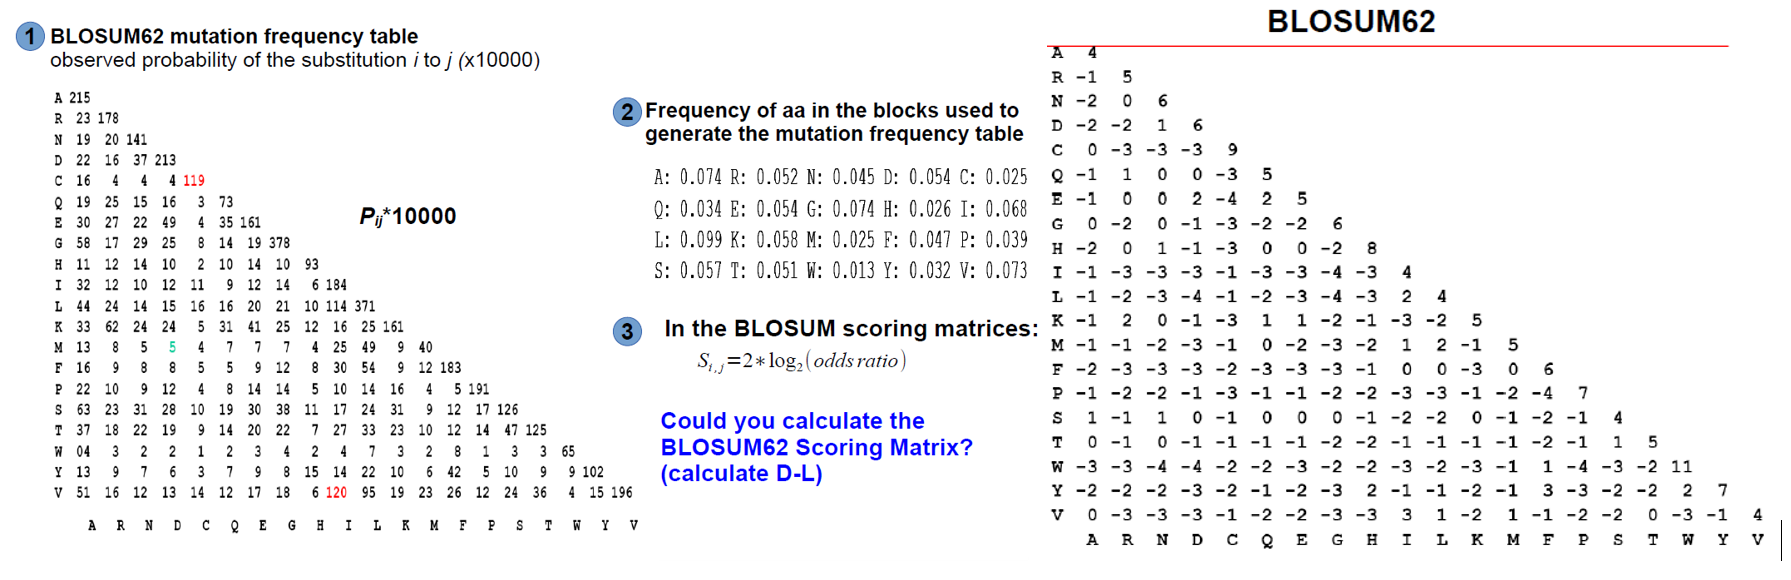
\includegraphics[width = \textwidth]{figs/ejercicio-blosum.png}
%\end{figure}

\subsubsection{Ejercicio}
\textit{\textbf{Ejercicio 1:} Queremos hacer una matriz de puntuación de ADN a partir de alineaciones de secuencias de ADN que muestren un 88\% de identidad (es decir, una matriz optimizada para encontrar alineaciones con un 88\% de identidad). Supongamos que todos los desajustes son equiprobables, y que la composición tanto de los alineamientos como de las secuencias de fondo es uniforme al 25\% para cada nucleótido. Construya la matriz de probabilidad de mutación y la matriz de puntuación. Introduzca los valores para la Matriz de Probabilidad de Mutación.}

Sabemos que las secuencias muestran un 88\% de identidad. Por tanto, en un 88\% de las ocasiones, las dos secuencias tienen los mismos residuos en la misma posición. Como cada nucleótido es equiprobable, $0,88/4 = 0,22$. Eso nos deja con $1 - 0,88 = 0,12$ a repartir entre los mismatches. Hay 12 posibilidades (12 casillas), y como todos son equiprobables, $0,12 / 12 = 0,01$. Ahora queda rellenar la tabla:

\begin{table}[htbp]
    \centering
    \begin{tabularx}{\textwidth}{ X | X X X X}
          & A & C & G & T \\ \hline
         A & 0,22 & 0,01 & 0,01 & 0,01 \\
         C & 0,01 & 0,22& 0,01 & 0,01 \\
         G & 0,01 & 0,01 & 0,22 & 0,01 \\
         T & 0,01 & 0,01 & 0,01 & 0,22 \\
    \end{tabularx}
\end{table}

En cuanto a la matriz de puntuación, nos indican que:
$$score = log_2(odds-ratio) = log_2(\frac{observado}{esperado})$$

El valor observado es aquel que obtenemos de la matriz de sustitución. El valor esperado es la probabilidad de los nucleótidos en ambas secuencias. Como una posición tendrá dos residuos (uno de cada secuencia), y todos los residuos son equiprobables, el valor esperado en cada caso será de $0,25 \cdot 0,25 = 0,0625$. Por ejemplo:

$$p_{AA} = log_2(\frac{0,22}{0,0625}) = 1,8 \approx 2$$
$$p_{AC} = log_2(\frac{0,01}{0,0625}) = -2,64 \approx -3$$

Así, la tabla resultante sería:

\begin{table}[htbp]
    \centering
    \begin{tabularx}{\textwidth}{ X | X X X X}
          & A & C & G & T \\ \hline
         A & 2 & -3 & -3 & -3 \\
         C & -3 & 2& -3 & -3 \\
         G & -3 & -3 & 2 & -3 \\
         T & -3 & -3 & -3 & 2 \\
    \end{tabularx}
\end{table}

%07/10
\subsection{Alineamientos de puntuación (scoring alignments)}
Las matrices de sustitución ofrecen un método para puntuar posiciones individuales. Sin embargo, para comparar diferentes alineaciones, necesitamos un único valor que represente la puntuación combinada de todas las posiciones. Para calcular dicha puntuación, suponemos que cada posición del alineamiento es independiente de las demás \footnote{Nótese que esto es probablemente una simplificación excesiva porque en las proteínas reales a menudo existe una correlación entre residuos adyacentes. Por ejemplo, en una hélice anfipática los residuos polares e hidrófobos se distribuyen en caras opuestas. Por lo tanto, habrá cierta correlación entre los residuos en ciertas posiciones.} y calculamos la puntuación del alineamiento S como la suma de las puntuaciones individuales de cada una de las n posiciones, siendo s la entrada de la matriz de sustitución para los residuos a y b en la posición i.

$$S = \sum_{i = 1}^{n} (s_{a,b})_i$$

En otras palabras, se pueden sumar los valores de las matrices BLOSUM de cada posición al haber utilizado el logaritmo. Ahora, esta función de puntuación sólo funciona para coincidencias y discordancias pero no tiene en cuenta los INDELs. Para representar los INDEL, un residuo o una serie de residuos en una secuencia de la alineación se empareja con guiones («-») en la otra secuencia. Durante la puntuación, la presencia de un hueco en el alineamiento da lugar a una penalización por hueco que se resta de la puntuación total. Hay dos razones para penalizar los huecos. En primer lugar, un hueco implica una diferencia entre las secuencias comparadas y, por tanto, reduce nuestra certeza sobre su origen común. Los huecos corresponden a eventos de inserción/deleción que ocurrieron durante la evolución desde el ancestro común en uno de los linajes. Por lo tanto, en general, cuanto mayor sea el número de huecos, mayor será la distancia evolutiva entre las secuencias. La segunda razón es que, introduciendo un número ridículo de huecos, podríamos aumentar artificialmente el número de coincidencias y, como consecuencia, aumentar la puntuación del alineamiento, aunque el alineamiento resultante no tendría sentido desde el punto de vista biológico. Así, las penalizaciones por huecos actúan limitando la introducción de huecos. Por lo general, el usuario establece la penalización por hueco a partir de un conjunto de valores predefinidos \footnote{En algunos programas, la penalización por hueco varía en función del tipo de residuo con el que se alinea el hueco. La razón es que algunos residuos tienden a estar fuertemente conservados debido a su impacto en la estructura/función. Por lo tanto, es más probable que la supresión de esos residuos altere la estructura/función y, por lo tanto, sufra selección negativa.} que se han determinado empíricamente a partir de la observación de su efecto en los alineamientos.

Otro aspecto a considerar es la longitud del hueco. Una forma de abordarlo es el esquema de \textbf{puntuación lineal de huecos}. Si $\delta$ es la penalización por la inserción o eliminación de un único símbolo, entonces $\kappa \delta$ sería la penalización por un hueco de longitud $\kappa$. Sin embargo, este modelo de costes implica que $\kappa$ huecos independientes tienen la misma penalización que un único hueco de longitud $\kappa$, lo que es inadecuado desde una perspectiva evolutiva. Los INDEL son el resultado de errores durante la replicación o reparación del ADN que provocan la limitación de un tramo de nucleótidos. Por tanto, una brecha, independientemente de su longitud, suele derivarse de un único evento de mutación, mientras que las brechas independientes surgieron por diferentes eventos de mutación.

En consecuencia, los \textbf{modelos de puntuación de huecos afines} diferencian la penalización por hueco abierto, la penalización aplicada la presencia de cada hueco independiente, y la penalización por extensión del hueco, que es menor que la anterior y es lineal con la longitud del hueco. La penalización por hueco afín se calcula a partir de estas dos penalizaciones diferentes como:

$$\delta + (\epsilon \cdot \kappa)$$

donde $\delta$ es la penalización por hueco abierto, $\epsilon$ la penalización por hueco extendido y $\kappa$ la longitud del hueco \footnote{Dependiendo del esquema de puntuación, $\kappa$ es la longitud del gap o la longitud del gap menos 1.} (número de residuos eliminados/insertados, es decir, guiones en la alineación). La penalización por hueco afín es el modelo de puntuación más popular. Impone una penalización mayor a los huecos más grandes. Aunque una brecha grande implica obviamente más diferencias a nivel de secuencia que una brecha más pequeña, ambas se produjeron como consecuencia de un único evento de mutación. Por este motivo, también se ha desarrollado una \textbf{puntuación constante de las diferencias}, que aplica una penalización a toda la diferencia, independientemente de su longitud.

Ahora podemos incorporar la penalización por hueco a la puntuación de alineación. La puntuación total del alineamiento se sigue calculando como la suma de las puntuaciones parciales en cada posición, de modo que para las coincidencias o discordancias utilizamos el valor $s_{a,b}$ de la matriz de sustitución y en los casos en que el símbolo de una de las secuencias sea un guión aplicamos la penalización por hueco. Definimos $\sigma_{a,b}$ como la función

$$\sigma (a, b) = \begin{cases}
s_{a,b} & \text{cuando} a \wedge b \neq gap \\
GapPenalty & \text{cuando} a \vee b = gap
\end{cases} $$

Y la puntuación del alineamiento como:

$$S = \sum_{i = 1}^{n} (\sigma(a,b))_i$$

\begin{table}[htbp]
\begin{mdframed}[backgroundcolor=black!10]
En resumen, hay consenso que, cuantos más gaps hay, más penalización debe recibir. Sin embargo, no hay consenso en cuanto a la penalización de los gaps, y hay tres esquemas:
\begin{itemize}
\item \underline{Gap penalty constante}: solo se tiene en cuenta si se ha abierto un gap, independientemente de su longitud.
\item \underline{Gap penalty linear}: se tiene en cuenta la extensión o longitud del gap.
\item \underline{Gap penalty afín}: Se tiene en cuenta si se ha abierto un gap y su longitud. Este esquema es el que se suele utilizar.
\end{itemize}

De esa forma, si los residuos a y b son, en un alineamiento, diferentes a "-" (es decir, no son gaps), se utiliza la matriz de sustitución. Si a o b son un gap, se emplea el gap penalty. 
\end{mdframed}
\end{table}

\begin{figure}
\centering
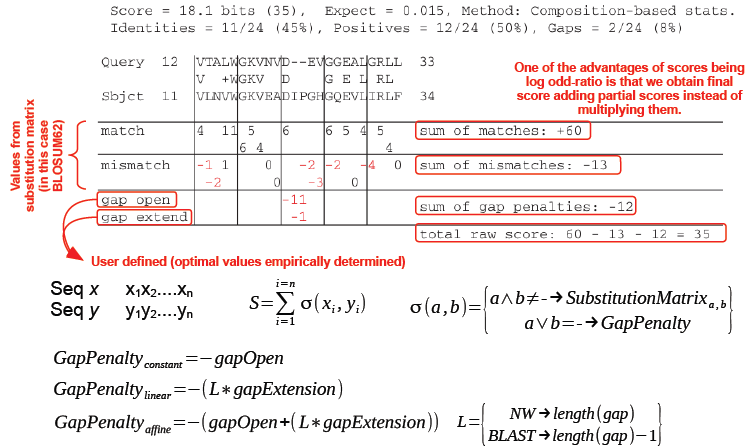
\includegraphics[width = \textwidth]{figs/gap-penalty.png}
\caption{Ejemplo de alineamiento con matriz de sustitución. Se han separado los valores de match y mismatch simplemente porque no cabían todos en línea. Los valores de penalización de apertura y extensión de gap los define el usuario de forma empírica. La longitud del gap se calcula de forma distinta en el algoritmo de Needleman-Wunsch que en BLAST.}
\end{figure}

\subsubsection{Ejercicio}
Calcula la puntuación del siguiente alineamiento: \\
TCCGGGGATCCCC-AGCA 17\\
TC--GGGATCCCCCATCA 16\\ 
Utilizando la siguiente matriz de puntuación:

\begin{table}[htbp]
    \centering
    \begin{tabularx}{\textwidth}{ X X X X X}
          & A & C & G & T \\ \hline
         A & +1 & -4 & -4 & -4 \\
         C & -4 & +1 & -4 & -4 \\
         G & -4 & -4 & +1 & -4 \\
         T & -4 & -4 & -4 & +1 \\
    \end{tabularx}
\end{table}

y penalización de gap de acuerdo con la expresión $G+L \cdot n$, donde G y L son las penalizaciones de existencia y extensión respectivamente y n la longitud del gap. En este caso, considera que la existencia (G) es 5 y la extensión (L) es 2. 

En este caso, la puntuación del alineamiento sería de:
$$+1 +1 -(5 +2 \cdot 2) +1 +1 +1 +1 +1 +1 +1 +1 +1 -(5 +2 \cdot 1) +1 -4 +1 +1 = -6$$

\subsection{Algoritmos de alineamiento}
Una vez que tengamos un método de puntuación, podríamos encontrar la alineación óptima entre dos proteínas enumerando todas las alineaciones posibles y eligiendo la de mejor puntuación. Sin embargo, este \textbf{enfoque de fuerza bruta} es poco práctico en términos de tiempo. El número de alineaciones posibles para dos secuencias de longitud m y n es $m^n$. Esto significa que un ordenador tiene que hacer un número de cálculos proporcional a $m^n$ para encontrar el alineamiento óptimo utilizando este enfoque de fuerza bruta. Así, pueden producirse más de $10^209$ alineaciones diferentes entre dos proteínas de tamaño medio (unos 350 residuos). Incluso procesando varios miles de alineaciones por segundo, el proceso duraría más que la edad del universo utilizando los ordenadores actuales. Afortunadamente, los bioinformáticos han encontrado formas inteligentes de reducir el tiempo de cálculo necesario para encontrar el mejor alineamiento posible, como se explica en las secciones siguientes.

\subsubsection{Algoritmos, complejidad del tiempo y notación de la big-O}
Un algoritmo puede definirse vagamente como un conjunto de pasos que pueden seguirse para alcanzar un objetivo. El conjunto de reglas que aprendiste en la escuela para multiplicar dos números largos es un ejemplo de algoritmo. El algoritmo define los pasos necesarios en un nivel abstracto; para que un ordenador siga los pasos, el algoritmo debe implementarse en un programa informático concreto. Así, un programa es la implementación de un algoritmo diseñado para realizar una tarea específica. En informática, la complejidad temporal describe el tiempo que se tarda en ejecutar un algoritmo. Dado que la velocidad de los distintos ordenadores varía, la complejidad temporal suele estimarse contando el número de pasos elementales que realiza el algoritmo, en lugar de en tiempo real. 

Los informáticos utilizan la notación big-O para describir de forma concisa el tiempo de ejecución de un algoritmo. En concreto, describe cómo crece el tiempo necesario para realizar el cálculo en función del tamaño de la entrada. 

\begin{figure}[htbp]
\centering
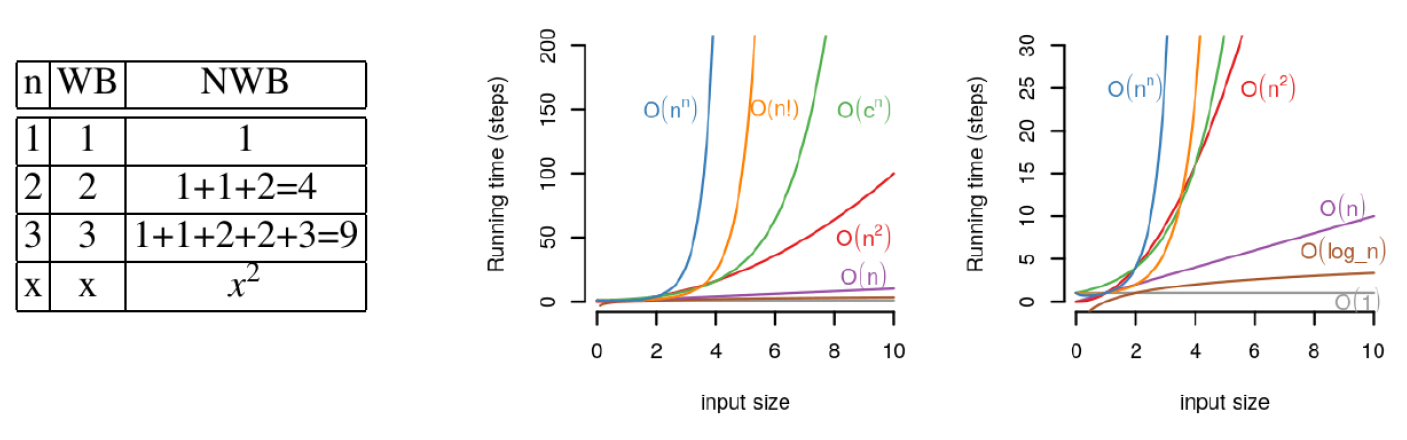
\includegraphics[width = \textwidth]{figs/big-o.png}
\caption{\textbf{Complejidad del tiempo y notación O grande}. La tabla a la izquierda de la figura muestra la comparación de los tiempos de carrera con y sin carretilla. El número de pasos que el trabajador debe caminar para construir una cerca de la longitud indicada ((n)) utilizando los algoritmos “carretilla” ((WB)) y “no carretilla” ((NWB)). Los gráficos de la derecha muestran la comparación de los tiempos de ejecución de algoritmos con diferentes complejidades temporales. Cada gráfico representa el número de pasos (eje y, "tiempo de ejecución") en función del tamaño de la entrada (eje x) para algoritmos con la complejidad de tiempo indicada: O(1), tiempo constante; O(log(n)), tiempo logarítmico; O(n), tiempo lineal; O($n^2$), tiempo cuadrático; O($c^n$) donde c es una constante, tiempo factorial; O(n!), tiempo factorial; O($n^n$), tiempo. Ambos gráficos son idénticos excepto por el valor máximo del eje y.}
\label{fig:big-O}
\end{figure}

Un ejemplo de juguete puede ser útil para comprender estos conceptos. Imaginemos que un trabajador construye una valla con ladrillos grandes. Si el trabajador utiliza una carretilla para transportar los ladrillos, el número de pasos (pasos físicos) que debe dar para construir la valla sería proporcional a la longitud de la valla. En este caso decimos que el «algoritmo» para construir la valla tiene una complejidad temporal lineal. Esto significa que si para una valla de 10 m de longitud el trabajador debe caminar un total de x pasos, para una valla de 50 m debe caminar 5x pasos. Imagina ahora que el trabajador no tiene carretilla. En este caso, debe coger el primer ladrillo, caminar y pasos para colocarlo y, a continuación, retroceder y pasos hasta el origen para coger el segundo ladrillo. Para colocar el segundo ladrillo, camina 2y para colocarlo más 2y pasos de vuelta al origen para coger el siguiente ladrillo, etc. La figura \ref{fig:big-O} compara el número de pasos de cada «algoritmo» en función del “tamaño de la entrada” que, en este ejemplo de juguete, es la longitud de la valla. El algoritmo «sin carretilla» muestra una complejidad temporal cuadrática, porque el número de pasos es proporcional al cuadrado del tamaño de la entrada. Usando la notación big O, «carretilla» es un algoritmo con complejidad temporal O(n), donde n es el tamaño de la entrada, mientras que «sin carretilla» es un algoritmo con complejidad temporal O($n^2$). Aunque ambos algoritmos darán el mismo resultado, «sin carretilla» tardará más que «carretilla» para cualquier longitud de valla (excepto n=1). Además, cuanto más larga sea la entrada (longitud de la valla a construir), mayor será la diferencia en pasos y, por tanto, en tiempo de ejecución (véase la figura \ref{fig:big-O}).

\subsubsection{Análisis de matriz de puntos (dot matrix alignment)}
Es el método más sencillo para comparar similitudes entre dos secuencias. Aunque es un método visual que no proporciona el alineamiento real, se utiliza a menudo para evaluar rápidamente, de un vistazo, la similitud entre dos secuencias. En este método, una de las secuencias se sitúa en el eje horizontal de una matriz con celdas vacías y la otra secuencia en el vertical. A continuación, cada uno de los residuos de una de las secuencias se compara con todos los residuos de la otra y se coloca un punto en la celda situada en la intersección de ambos residuos siempre que se produzca una coincidencia (residuo idéntico o similar en ambas secuencias). En esta representación, las regiones similares (tramos alineados de la secuencia) se muestran como diagonales en la matriz (véase la figura \ref{fig:dotplot}). El análisis de la matriz de puntos puede revelar fácilmente la presencia de inserciones/deleciones (huecos en la diagonal principal) y repeticiones directas/invertidas (diagonales paralelas/perpendiculares a la principal).

\begin{figure}[htbp]
\centering
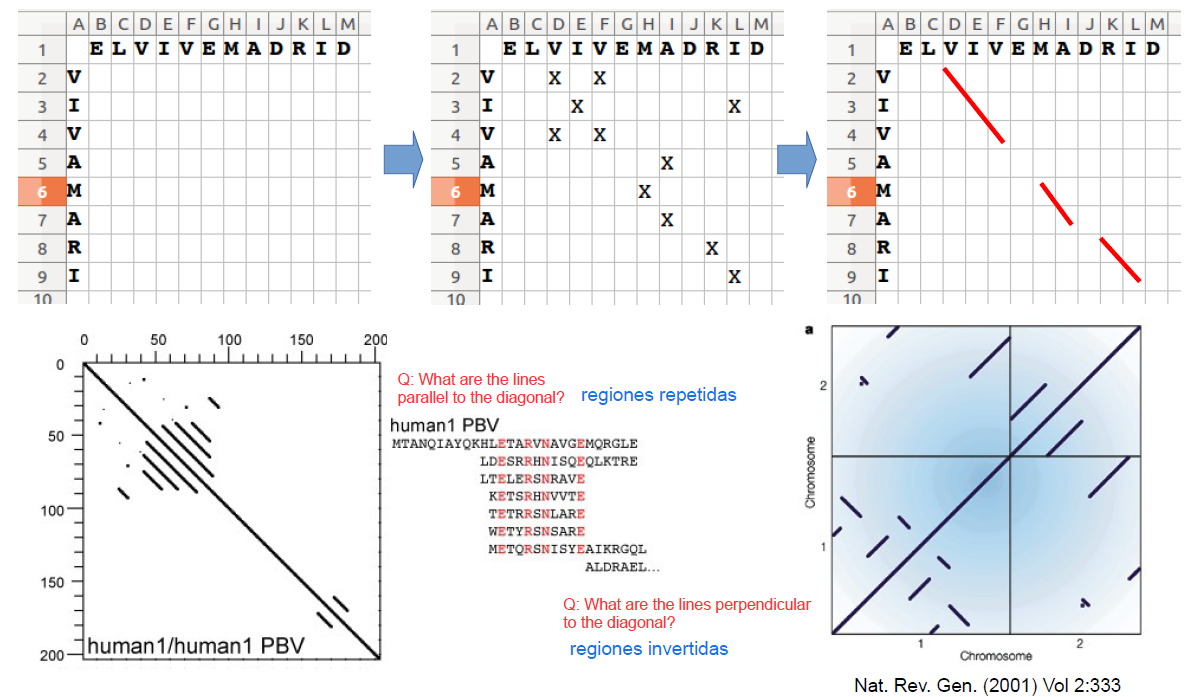
\includegraphics[width = \textwidth]{figs/dot-plot.png}
\caption{\textbf{Alineación matricial de puntos.} En su versión más sencilla, el análisis de matriz de puntos rellena una matriz de 2 dimensiones con coincidencias entre residuos de ambas secuencias y une las celdas diagonales adyacentes para producir el gráfico. La figura indica los pasos para producir el gráfico de izquierda a derecha. Las identidades se muestran en rojo oscuro y las similitudes en rojo claro.}
\label{fig:dotplot}
\end{figure}

\subsubsection{Programación dinámica}
Como ya se ha comentado, encontrar el mejor alineamiento posible mediante un algoritmo de fuerza bruta tiene una complejidad temporal de O($m^n$), lo que resulta poco práctico para alineamientos que impliquen más de unos pocos residuos. Afortunadamente, los algoritmos \textbf{Needleman-Wunsch} y \textbf{Smith- Waterman} son capaces de calcular el alineamiento óptimo entre dos proteínas en un tiempo muy ordenado. La diferencia entre ellos es que \textbf{Needleman-Wunsch calcula el alineamiento global} entre las proteínas, mientras que \textbf{Smith-Waterman produce alineamientos locales}. Los alineamientos globales contienen los residuos de las dos secuencias que se están alineando. Por el contrario, los alineamientos locales tratan de encontrar la región o regiones de mayor similitud entre las dos secuencias y producen un alineamiento (o varios) que contienen sólo los residuos incluidos en la región de alta similitud despreciando el resto de la secuencia. Los alineamientos locales son importantes para identificar regiones de gran similitud entre secuencias que, de otro modo, no comparten mucha identidad. Dado que las proteínas son modulares, es decir, contienen diferentes dominios funcionales, el alineamiento local permite identificar dominios compartidos entre proteínas con diferentes arquitecturas de dominio (figura \ref{fig:global-local}). Por ejemplo, aunque existen muchas proteínas quinasas diferentes pertenecientes a distintas familias, todas ellas contienen un dominio quinasa. Sin embargo, este dominio suele estar combinado con otros dominios que son específicos de cada familia de quinasas. Las quinasas AKT contienen un dominio de homología Pleckstrine (PH), necesario para la unión de fosfoinositidos, que se encuentra N-terminal al dominio quinasa. En cambio, las proteínas cinasas dependientes de cGMP contienen dos regiones de unión a cGMP, pero no un dominio PH, N-terminal a su dominio cinasa. No tendría mucho sentido intentar un alineamiento global entre estas dos quinasas, pero un alineamiento local revelaría una fuerte región de similitud correspondiente al dominio quinasa. 

\begin{figure}[htbp]
\centering
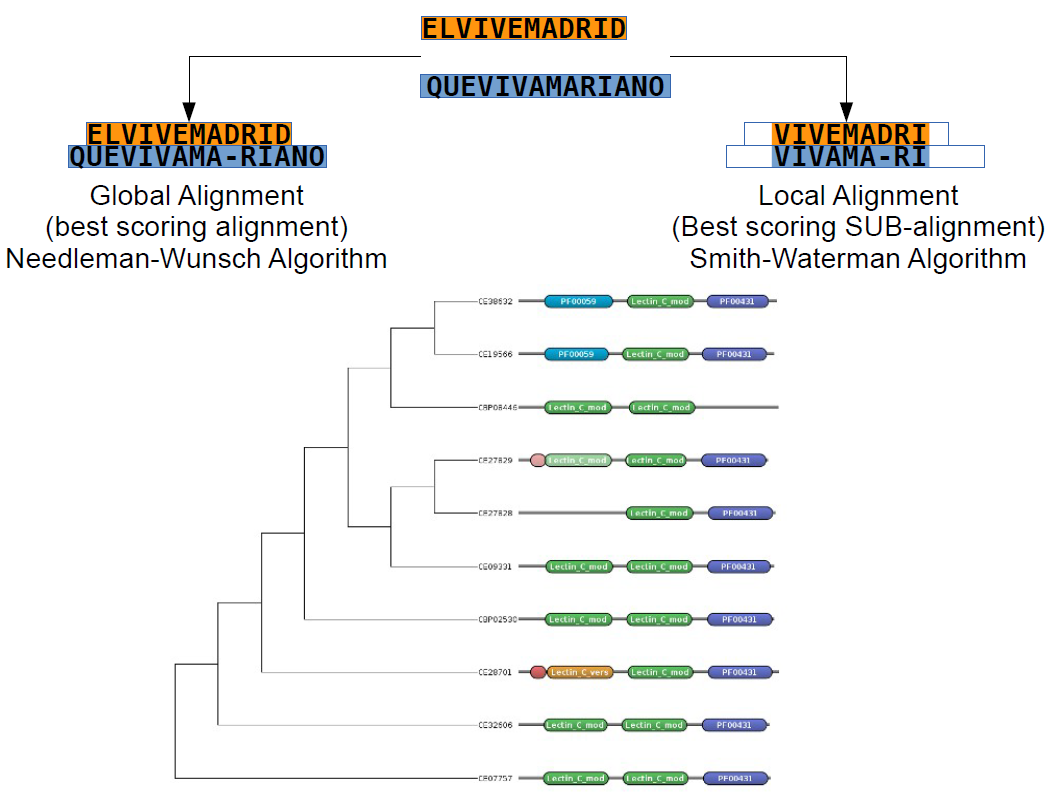
\includegraphics[width = 0.65\textwidth]{figs/alineamientos-global-local.png}
\caption{Comparación de un alineamiento global y local y su representación gráfica con los dominios de distintas proteínas.}
\label{fig:global-local}
\end{figure}

Ambos algoritmos, el de Needleman-Wunsch y el de Smith-Waterman, se basan en un método computacional llamado \textbf{programación dinámica}, que garantiza proporcionar el alineamiento óptimo (es decir, el mejor o el de mayor puntuación) para un par dado de secuencias en un tiempo proporcional a n $\cdot$ m (puesto que m $\approx$ n, entonces O($n^2$), es decir, tiempo cuadrático). Como se muestra en la figura \ref{fig:big-O}, estos algoritmos son mucho más rápidos, lo que permite calcular el alineamiento óptimo de forma práctica. Es importante destacar que los algoritmos de programación dinámica proporcionan la mejor alineación posible de acuerdo con un conjunto dado de reglas (puntuación por una coincidencia y penalizaciones por coincidencias erróneas y huecos), es decir, de acuerdo con un modelo matemático para la alineación de secuencias. Sin embargo, no se garantiza que el alineamiento óptimo resultante sea biológicamente relevante. Obsérvese que incluso para dos secuencias aleatorias el algoritmo informará de su mejor (aunque en este caso biológicamente irrelevante) alineación posible.

Al utilizar un algoritmo de programación dinámica, el número de comparaciones necesarias se reduce drásticamente. Además, al calcular todos los alineamientos posibles entre dos secuencias hay algunas operaciones (comparación entre residuos concretos) que se repiten una y otra vez. La programación dinámica mantiene un registro de todos esos cálculos en una tabla, por lo que evita la repetición, lo que supone un enorme ahorro de tiempo. En resumen, al calcular todos los alineamientos posibles, muchos subalineamientos se repiten muchas veces. La programación dinámica guarda el resultado de cada cálculo parcial para que, si se necesita más adelante, no haya que repetirlo. 

\begin{figure}[htbp]
\centering
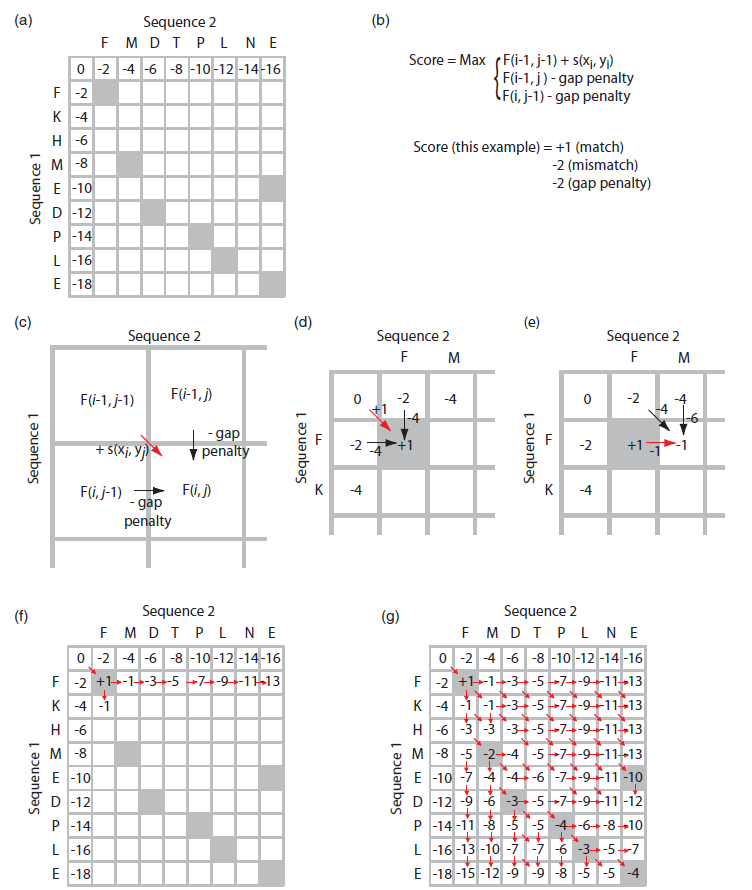
\includegraphics[width=0.8\textwidth]{figs/programacion-dinamica.png}
\caption{\small \textbf{Alineación por pares de dos secuencias de aminoácidos utilizando el algoritmo de programación dinámica de Needleman y Wunsch para el alineamiento global.} (a) Para secuencias de longitud m y n formamos una matriz de dimensiones m + 1 por n + 1 y añadimos penalizaciones por huecos en la primera fila y columna. Cada posición de hueco recibe una puntuación de -2. Las celdas que tienen identidad están sombreadas en gris. (b) El sistema de puntuación en este ejemplo es +1 para una coincidencia, -2 para una falta de coincidencia y -2 para una penalización por hueco. En cada celda, la puntuación se asigna utilizando el algoritmo recursivo que identifica la puntuación más alta a partir de tres cálculos. (c) En cada celda F(i, j) calculamos las puntuaciones derivadas de seguir un camino desde la celda superior izquierda (sumamos la puntuación de esa celda + la puntuación de F(i, j)), la celda de la izquierda (incluyendo una penalización por hueco) y la celda inmediatamente superior (de nuevo incluyendo una penalización por hueco). (d) Para calcular la puntuación de la celda de la segunda fila y columna, tomamos la máxima de las tres puntuaciones +1, -4, -4. Esta mejor puntuación (+1) sigue la trayectoria de la flecha roja, y mantenemos la información de la mejor trayectoria, resultante en la puntuación de cada celda para reconstruir posteriormente la alineación por pares. (e) Para calcular la puntuación de la segunda fila, tercera columna, volvemos a tomar el máximo de las tres puntuaciones -4, -1, -4. La mejor puntuación se obtiene a partir de la celda de la izquierda (flecha roja). (f) Procedemos a rellenar las puntuaciones de la primera fila de la matriz. (g) La matriz completada incluye la puntuación global del alineamiento óptimo (-4; véase la celda de abajo a la derecha, correspondiente al extremo carboxi de cada proteína). Las flechas rojas indican la(s) ruta(s) por la(s) que se obtuvo la puntuación más alta para cada celda.}
\label{fig:dynamic-programming}
\end{figure}

\normalsize
Para cada posición de un alineamiento, hay tres opciones posibles: que se alineen los residuos de ambas cadenas, que haya un gap en una cadena o que haya un gap en la otra cadena. La programación dinámica utiliza una matriz como la empleada en la figura \ref{fig:dynamic-programming}. Cuando se avanza de forma lateral (ya sea en horizontal o en vertical), se produce un gap en una u otra secuencia, mientras que cuando se avanza en diagonal, se produce el alineamiento de los dos residuos. Se rellena la matriz con las puntuaciones de cada uno de los movimientos y se marca aquel que sea más favorable. Si se produce alguna situación en la que haya dos valores máximos o iguales, es decir, dos direcciones que den el mismo score global, se escoge cualquiera de ellos ya que ambos alineamientos serían igual de buenos. El valor de la esquina inferior izquierda es el score global del alineamiento. Una vez rellena la matriz, se produce el alineamiento recorriendo el camino a la inversa siguiendo las direcciones más favorables. Un programa para calcular esto es \href{https://baba.sourceforge.net/}{BABA}, ya que permite introducir las secuencias, ajustar las penalizaciones por gaps e ir viendo cómo se rellena la matriz paso a paso. En este programa, las flechas están al revés, ya que indican de dónde vienen en lugar de a dónde van.

\begin{table}[htbp]
\begin{mdframed}[backgroundcolor=black!10]
\textbf{[Material adicional] Obtener el número de alineamientos posibles con gaps:} Las tres posibles formas de moverse en la matriz se puede resumir en dos vectores. El número de pasos que dar es la suma de los pasos que se dan desde el inicio al final del alineamiento. Sumando todos los caminos, se tendría el número de alineamientos posibles. El número de matches es igual al número de vectores (1,1). Para obtener el valor total, se utilizan los números combinatorios. Para calcular el número total global de todos los alineamientos, es el sumatorio de k (matches posibles) y el número mínimo de m y n.

$$\sum_{k=0}^{min(m,n)} = \begin{pmatrix}
          m + n - k \\
          k, m-k, n-k
    \end{pmatrix}$$
\end{mdframed}
\end{table}

\subsection{Relevancia estadística de la puntuación de alineamiento}
Los métodos de alineación devolverán la mejor coincidencia posible entre dos secuencias dadas. Sin embargo, es de vital importancia tener en cuenta que, dadas dos secuencias cualesquiera, los algoritmos de alineación siempre devolverán una alineación que sea la mejor posible según un conjunto de reglas matemáticas (el esquema de puntuación). Sin embargo, \textbf{ser el mejor posible no significa necesariamente que sea biológicamente relevante}. Por ejemplo, la proteína BAD (bcl2-associated agonist of cell death) es un miembro de la familia Bcl-2 y, como tal, un actor clave en el proceso de apoptosis, un tipo de muerte celular programada (PCD) bien caracterizado en animales. Aunque la PCD está documentada en plantas, la maquinaria responsable de impulsar el proceso sigue siendo esquiva y los reguladores apoptóticos, incluidos los miembros de la familia Bcl-2, aún no se han identificado en plantas. La figura \ref{fig:bad-thaliana} muestra la mejor coincidencia de la proteína BAD humana en la planta \textit{Arabidops thaliana}. Ahora bien, ¿es esta proteína putativa de \textit{A. thaliana} un verdadero homólogo de la proteína BAD humana o se trata simplemente de la mejor coincidencia posible según nuestro esquema de puntuación, aunque no tenga un ancestro común con BAD? 

\begin{figure}[htbp]
\centering
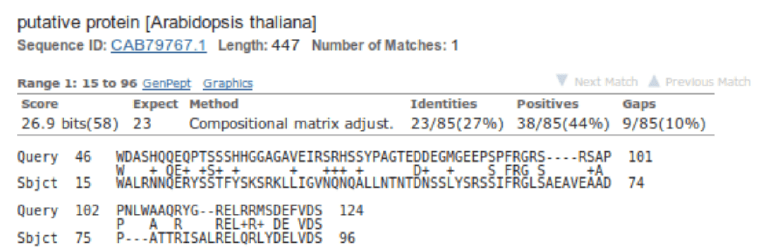
\includegraphics[width = \textwidth]{figs/bad-thaliana.png}
\caption{\textbf{¿Homólogo vegetal de BAD?} Alineación del mejor resultado de una búsqueda BLAST utilizando la proteína humana BAD (NP-004313.1) como consulta frente a las proteínas de \textit{Arabidopsis thaliana} (taxid:3702). El Expect se fijó en 100 y el resto de parámetros BLAST se dejaron con los valores por defecto.}
\label{fig:bad-thaliana}
\end{figure}

En el análisis de alineamientos de proteínas, la puntuación que se obtiene al comparar diferentes secuencias es clave para determinar la posible homología entre ellas (cuanto mayor sea la puntuación, mayor será la probabilidad de que las proteínas deriven de un ancestro común). Sin embargo, la mera comparación de puntuaciones no es suficiente para asegurar que las secuencias están relacionadas evolutivamente; es necesario un análisis estadístico más profundo para descartar que las similitudes observadas se deban al azar. En otras palabras, ¿cómo de grande debe ser la puntuación para que concluyamos que las proteínas son homólogas?
El concepto central es la \textbf{hipótesis nula}, que asume que el alineamiento observado es producto de secuencias no relacionadas (aleatorias). Para evaluar esta hipótesis, es necesario comparar la puntuación obtenida ($s_{ab}$) con la distribución de puntuaciones que se obtendrían al alinear proteínas no homólogas o generadas aleatoriamente. De esta manera, podemos calcular un \textbf{p-valor} empírico, que representa la probabilidad de obtener una puntuación igual o superior a la observada simplemente por azar. Este p-valor se calcula como la proporción de veces que un alineamiento aleatorio supera la puntuación observada, proporcionando una medida objetiva de la significancia del alineamiento.
Por otra parte, si la distribución de las puntuaciones aleatorias sigue una distribución estadística conocida (por ejemplo, una distribución normal), podemos aplicar las herramientas de la inferencia estadística para calcular el valor p exacto. Sea cual sea el método utilizado para calcular el valor p, empírico o exacto, indica la probabilidad de que la puntuación $s_{ab}$ se deba al azar. Podemos aceptar la alineación como significativa (posiblemente indicando homología) si su puntuación está en el 5\% superior (u otro valor elegido) de las puntuaciones generadas aleatoriamente (p <0,05).

Por ejemplo, al comparar las proteínas NP-508008 (proteína 1) y NP-29564 (proteína 2), el alineamiento obtuvo una puntuación de 55,5, mientras que al comparar NP-508008 con NP-001421 (proteína 3), el valor fue de 477. A pesar de que ambos alineamientos presentaban valores similares en identidad, similitud y gaps, las diferencias en las puntuaciones indican posibles diferencias evolutivas entre los pares de proteínas. Para evaluar la relevancia de estos scores, se realizó un alineamiento de la proteína 1 con una secuencia generada aleatoriamente, y los valores obtenidos fluctuaron entre 8,5 y 100. Dado que el valor 55,5 del alineamiento entre las proteínas 1 y 2 cae dentro de este rango, podemos inferir que la similitud observada podría deberse al azar y, por tanto, no hay evidencia clara de una relación evolutiva significativa entre ellas. Por otro lado, la puntuación de 477 para el alineamiento entre las proteínas 1 y 3 se encuentra fuera del rango de valores aleatorios, lo que sugiere una relación evolutiva significativa. El p-valor para el alineamiento de las proteínas 1 y 2 se calculó como 0,34 (34\%), lo que indica que el 34\% de los alineamientos aleatorios tienen puntuaciones iguales o superiores a 55,5. Dado que este valor es mayor que el umbral típico de significancia (p < 0,05), no se puede rechazar la hipótesis nula, lo que sugiere que la similitud observada es posiblemente un producto del azar. En cambio, en el caso del alineamiento entre las proteínas 1 y 3, no se observó ninguna puntuación aleatoria cercana a 477, lo que implica que la probabilidad de que esta similitud sea debida al azar es extremadamente baja. Por lo tanto, para concluir si dos secuencias están evolutivamente relacionadas no es suficiente con observar una alta puntuación en el alineamiento; es necesario calcular un valor estadístico como el p-valor que permita definir con precisión la relevancia de dicho alineamiento. En resumen, el algoritmo Needleman-Wunsch nos proporciona una herramienta para generar alineamientos óptimos, pero carece de la capacidad para distinguir si un alineamiento tiene o no base biológica, razón por la cual es crucial el uso de métodos estadísticos adicionales para interpretar correctamente los resultados.

%09/10 - Luis del Peso
\textbf{Ejercicio práctico (problema de programación):} Partiendo de un script que computa el alineamiento entre dos secuencias de aminoácidos, se debe modificarlo para calcular el p-valor empírico asociado al score del alineamiento.  Se deben dar dos secuencias de entrada, y se debe obtener un p-valor asociado al score como salida.

\subsection{Métodos basados en k-tuplas o palabras - alineamiento heurístico con BLAST} 
El alineamiento por pares rara vez se utiliza para comparar dos secuencias dadas, sino que suele emplearse para buscar en una base de datos con una secuencia de consulta para identificar secuencias similares. A pesar de la eficacia de los algoritmos de alineación basados en la programación dinámica, el gran tamaño de las bases de datos actuales haría que las búsquedas con estos métodos exactos fueran demasiado lentas \footnote{En las bases de datos biológicas, a día de hoy se estima que hay $10^8$ - $10^9$ residuos, y una proteína normal tiene $10^2$ - $10^3$ residuos. Así, la matriz de scoring tendría que tener $10^3$ residuos en un lado y $10^8$ en el otro, por lo que el rastreo tarda horas.}. Por este motivo se desarrollaron nuevas alternativas más rápidas a los métodos de programación dinámica: FASTA y el muy popular BLAST (Basic Local Alignment Search Tool). Para aumentar la velocidad de la búsqueda, estos programas no realizan un alineamiento exacto (es decir, óptimo) entre la consulta y cada una de las secuencias de la base de datos, sino que estos métodos primero escanean la base de datos en busca de posibles coincidencias y luego realizan un alineamiento más preciso con ellas. Sin embargo, la mayor velocidad tiene un precio. A diferencia de los métodos dinámicos, no se garantiza que FASTA y BLAST encuentren los alineamientos óptimos. Los métodos o algoritmos que cambian precisión por velocidad se denominan heurísticos. Así, FASTA y BLAST son \textbf{algoritmos heurísticos} que permiten buscar en bases de datos mucho más rápido que los métodos precisos, como Needleman-Wunsch y Smith-Waterman, pero que no garantizan devolver el mejor alineamiento posible (óptimo). La estrategia utilizada por FAST y BLAST para reducir el tiempo de búsqueda consiste en dividir la consulta en k-mers \footnote{En bioinformática, los k-mers son subsecuencias de longitud k contenidas en una secuencia más larga.} o palabras e identificar secuencias en la base de datos que contengan coincidencias exactas (o casi exactas) con cualquiera de los k-mers de la consulta. A continuación, se puntúan las coincidencias en la base de datos y las mejores se amplían mediante programación dinámica.
Una búsqueda en la base de datos con el algoritmo BLAST sigue estos pasos:
\begin{enumerate}
\item Hace una lista de todas las palabras k-mers contenidas en la secuencia de consulta. La longitud de la palabra se fija por defecto en 3 residuos (3-mer) para las búsquedas de proteínas y en 11 residuos (11-mer) para los ácidos nucleicos. No obstante, el valor del parámetro del tamaño de la palabra (word size) puede ser modificado por el usuario para adaptar la búsqueda a necesidades específicas. Cuanto menor sea el word size, mayor será la sensibilidad, pero requiere más semillas que extender y un mayor tiempo de computación. 
\item Para cada una de las palabras derivadas de la consulta, el algoritmo identifica todas las palabras similares que, según la matriz de sustitución elegida, darían lugar a una puntuación superior a un umbral predefinido en un alineamiento por pares. El umbral se obtiene por BLAST de forma empírica. Las palabras resultantes son las palabras de alta puntuación, HSW (high scoring words).
\item El algoritmo busca en las secuencias de la base de datos coincidencias exactas con cualquiera de las HSW. Cada coincidencia, denominada High-scoring Segment Pair (HSP), se utiliza en el siguiente paso para ampliar este alineamiento semilla.
\item Cada HSP identificado en el paso anterior se extiende entonces en ambas direcciones hasta que la puntuación total del HSP creciente comienza a disminuir.
\item Todos los HSP con una puntuación superior a un umbral predefinido se retienen y el BLAST calcula el alineamiento local Smith-Waterman entre la consulta y la secuencia objetivo en el HSP.
\end{enumerate}

\begin{figure}[htbp]
\centering
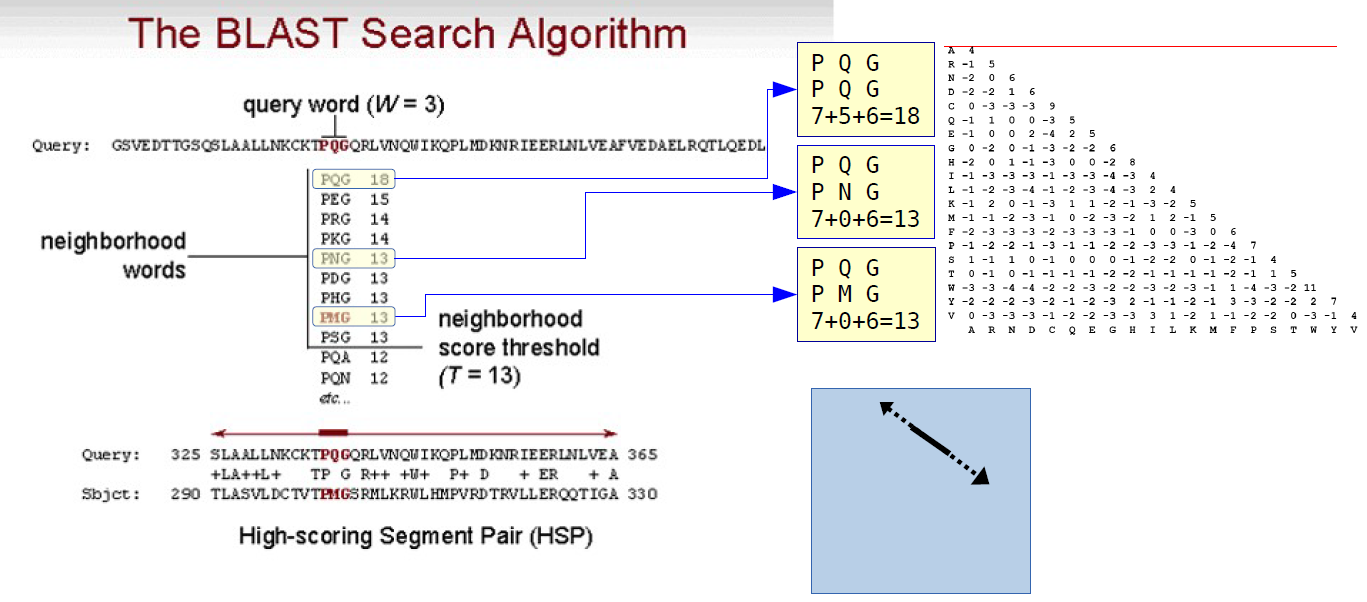
\includegraphics[width = \textwidth]{figs/blast-algorithm.png}
\caption{Ejemplo de una búsqueda mediante BLAST.}
\end{figure}

BLAST no informa de un valor p como tal, sino que proporciona el \textbf{valor E} o valor esperado (Expect value). BLAST se emplea normalmente para buscar en una base de datos con una consulta y el valor E es un parámetro que describe el número de resultados que uno puede "esperar" ver por casualidad al buscar en una base de datos de un tamaño determinado. Cuanto más bajo sea el valor E, más significativa será la puntuación y la alineación (se considera que un valor es significativo cuando el valor E es menor que $10^-4$). Además, el valor E disminuye si el tamaño de la base de datos disminuye (si solo se tiene cuenta una especie, por ejemplo). El valor E se relaciona con el valor p mediante la ecuación:
$$p = 1 - e^{-E}$$

El valor E en el alineamiento mostrado en la figura \ref{fig:bad-thaliana} es 23, lo que significa que se esperarían 23 alineamientos con una puntuación igual o mejor que 26,9 bits sólo por azar. Además, el valor p asociado es 1, por lo que no descartamos la hipótesis nula (la puntuación sí pertenece a la distribución aleatoria).

%11/10 - Luis del Peso
\textbf{Ejemplo práctico}: 
En BLAST, utilizamos la proteína humana EPAS1 (NP\_001421) contra la base de datos de Swissprot, restringiendo la búsqueda a \textit{Drosophila melanogaster}. El primer hit que sale es la proteína 	Q24167.2 con un E-valor de 9e-89 y una cobertura de 40\%. Como el E-valor es muy pequeño, sí se puede concluir que las dos proteínas son homólogas, pero no en toda su longitud (solo un dominio). No obstante, al realizar la búsqueda inversa, el primer hit es la proteína HIF1A humana, y no EPAS1 (ese es el segundo hit). Esto se debe a los genes parálogos, genes que en algún momento de la historia evolutiva se duplicaron y se siguen encontrando en el mismo genoma (por tanto, siguen siendo homólogos) y ortólogos, genes que han sufrido especiación, encontrándose así en genomas distintos. En humanos, hay tres genes parálogos llamados EPAS1, HIF1A y HIF3A, mientras que en \textit{Drosophila} solo hay una copia de este gen. En algún momento de la evolución de los vertebrados, el gen se triplicó. Lo más parecido con el gen de \textit{Drosophila} es HIF1A, por lo que se infiere que ese es el gen ancestral. En general, los genes ortólogos suelen ser los más similares. Esto se debe a que los genes esenciales tienen una presión selectiva a que no se modifiquen, mientras que en el caso de los parálogos, el gen duplicado permite acumular mutaciones al tener una copia que mantenga la función esencial. Así, la copia puede divergir y adquirir una nueva función. 

Así, cuando se realiza una búsqueda en BLAST, lo primero que hay que mirar es el E-value y si es menor o igual que $10^{-4}$. Después hay que mirar si ambos genes se encuentran en la misma especie (y son parálogos) o en distintas especies (y son ortólogos). No obstante, para poder determinar si un gen es el verdadero ortólogo de otro, hay que hacer el BLAST reverso; hay que realizar una nueva búsqueda con la secuencia que se cree que puede ser ortóloga y ver si aparece la secuencia anterior. Si esto es cierto, entonces sí se puede decir que las secuencias son verdaderas homólogas.

\begin{table}[htbp]
\begin{mdframed}[backgroundcolor=black!10]
\textbf{Similitud, identidad y homología}

Los términos similitud, identidad y homología se utilizan a veces de forma errónea. La similitud es un término descriptivo general que indica vagamente que las secuencias analizadas muestran cierto grado de coincidencia. La identidad se refiere al número de residuos idénticos que coinciden entre las secuencias alineadas. A diferencia de la similitud, la identidad es una medida objetiva. A menudo, utilizamos el porcentaje de identidad, que se define como el número de coincidencias idénticas dividido por la longitud de la región alineada y multiplicado por 100. La homología implica un antepasado común. Dos secuencias son homólogas si comparten un ancestro evolutivo común. Tenga en cuenta que homología es un término dicotómico, lo que significa que las secuencias son homólogas o no. Es un error común referirse al porcentaje de identidad como porcentaje de homología, este último carece de sentido. Dado que la homología implica un ancestro común, se suele suponer que las proteínas homólogas comparten una función y/o estructura común (o relacionada). Esto permite la anotación de proteínas recién encontradas sólo basándose en sus secuencias. En general, las proteínas homólogas tienden a mostrar una mayor similitud y un mayor porcentaje de identidad que las proteínas no relacionadas. Sin embargo, también está bien documentado que proteínas con muy poca similitud de secuencia entre sí pueden compartir una estructura y función similares. Así pues, un bajo porcentaje de identidad no excluye necesariamente la homología ni implica una función o estructura diferentes. Asimismo, secuencias con orígenes evolutivos diferentes pueden tener la misma función biológica como resultado de la evolución convergente. Sin embargo, dado que la evolución convergente no suele dar lugar a una similitud significativa de las secuencias, un alineamiento con una puntuación elevada suele implicar homología (es decir, la elevada similitud es consecuencia de un origen evolutivo común y no de la evolución convergente de dos secuencias de orígenes diferentes).
\end{mdframed}
\end{table}

\subsection{Interpretación biológica de alineamientos de secuencia: identificación de secuencias afines}
Como ya hemos mencionado, uno de los usos más importantes del alineamiento de secuencias es la búsqueda en bases de datos con el objetivo de identificar secuencias relacionadas con una consulta. Se considera que las secuencias similares están conservadas evolutivamente, es decir, que derivan de un ancestro común y, por tanto, deberían tener una estructura/función similar. Sin embargo, una vez que tenemos un alineamiento, ¿cómo decidimos (basándonos en él) si las secuencias están relacionadas o no? En otras palabras, ¿cuán similares deben ser dos secuencias para ser consideradas homólogas? Evidentemente, cuanto mayor sea el porcentaje de residuos similares, mayor será la probabilidad de que sean homólogas. El límite inferior suele fijarse en el 25-30\% de identidad para las secuencias de aminoácidos y en más del 70\% para las de nucleótidos. Es importante señalar que esas recomendaciones se aplican a secuencias de más de 100 residuos, ya que es probable encontrar un alineamiento de alta puntuación con consultas de secuencias cortas. Por debajo de este umbral se encuentra una región, denominada \textbf{Twilight zone}, en la que no podemos estar seguros de que las similitudes encontradas sean relevantes. Desde una perspectiva estadística, la inspección de las identidades porcentuales tiene una utilidad limitada en la Twilight zone (identidad inferior al 25\%) porque no proporciona un conjunto riguroso de reglas para inferir homología, y se asocia con resultados falsos positivos o falsos negativos. En ocasiones, un alto grado de identidad en una región corta podría no ser evolutivamente significativo y, a la inversa, un bajo porcentaje de identidad podría reflejar homología. Así pues, el porcentaje de identidad por sí solo no basta para demostrar (ni para descartar) la homología. Hay dos factores de confusión que debemos tener en cuenta al utilizar el porcentaje de identidad para evaluar la homología. El primero es la \textbf{longitud de las secuencias alineadas}. No es lo mismo observar un 25\% de identidad sobre 150 residuos que sobre 10. El segundo es la \textbf{distancia evolutiva}, obviamente dos homólogos realmente distantes compartirán un porcentaje de identidad menor que dos homólogos cercanos. Así pues, el porcentaje de identidad en sí mismo no es un criterio suficientemente sólido para evaluar la homología. A pesar de ello, algunos investigadores han sugerido que si dos proteínas comparten un 25\% o más de identidad de aminoácidos en un intervalo de 150 o más aminoácidos, es probable que estén significativamente relacionadas, y si dos proteínas comparten un 20\% - 25\% de identidad en un tramo razonablemente largo (por ejemplo, de 70 a 100 residuos de aminoácidos), se encuentran en la Twilight zone. Sin embargo, es importante tener en cuenta que dos proteínas que no están relacionadas en absoluto suelen compartir entre un 10\% y un 20\% de identidad por casualidad cuando se alinean.

\begin{figure}
\centering
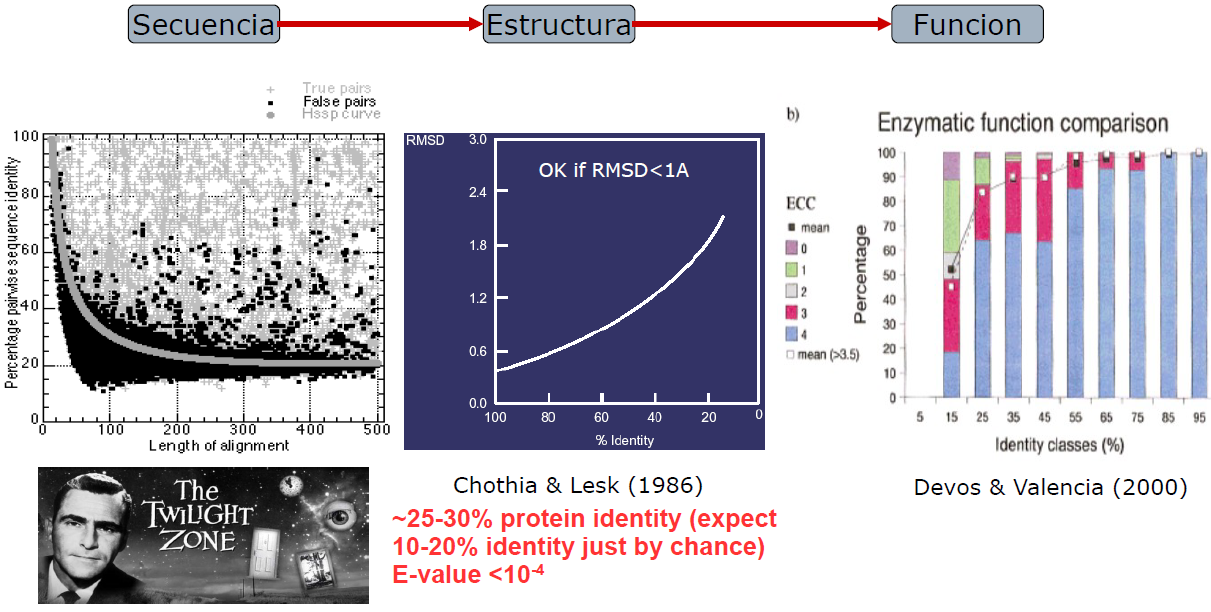
\includegraphics[width = \textwidth]{figs/twilight-zone.png}
\caption{Representaciones gráficas de la Twilight Zone.}
\end{figure}


%11/10 - Luis del Peso
\chapter{Alineamiento de múltiples secuencias (MSA)}
¿Cuál es la ventaja del MSA frente a los alineamientos por pares? La principal ventaja es que hay mucha más información en un MSA que en un alineamiento por pares, por lo que al realizar un MSA mejoramos la relación señal/ruido. Consideremos el ejemplo de juguete de la figura \ref{fig:msa}. Muestra la alineación de un fragmento del dominio Ser/Thr-quinasa del AK77 humano con dos proteínas de archaea. Ambas alineaciones por pares son relativamente similares, por lo que sería difícil decidir cuál de ellas, si es que hay alguna, representa un verdadero homólogo de la consulta (los valores E son $3 \cdot 10^6$ y $7 \cdot 10^7$ respectivamente). Además, incluso sabiendo que el segundo alineamiento corresponde a un verdadero homólogo, sería difícil identificar qué residuos son esenciales para la actividad y/o el plegamiento del dominio quinasa. Sin embargo, un MSA de miembros de la familia Ser/Thr-quinasa revela los residuos clave del dominio catalítico. Además, esta información indica que el primer alineamiento corresponde a un falso positivo. Esto significa que, a pesar del valor E relativamente bajo, es poco probable que las proteínas alineadas compartieran un ancestro común. Este ejemplo también muestra que el MSA de un grupo de secuencias homólogas define los dominios o motivos que caracterizan a una familia de proteínas. Los residuos alineados en un MSA se derivan presumiblemente de un ancestro común, es decir, son homólogos en un sentido evolutivo. En consecuencia, los residuos conservados en un MSA tienden a ocupar posiciones correspondientes en la estructura tridimensional de cada una de las proteínas homólogas. Es importante señalar que las estructuras tienden a estar más conservadas que las secuencias dentro de una familia de proteínas. Así, para dos proteínas homólogas distantes, la conservación a nivel de residuos podría ser baja, por ejemplo un 30\% de identidad, mientras que tienen una proporción mucho mayor de residuos, por ejemplo un 50\%, localizados en posiciones equivalentes de sus estructuras tridimensionales. En consecuencia, los verdaderos homólogos distantes suelen tener una función bioquímica/biológica similar a pesar de la baja identidad de secuencia. Y lo que es más importante, utilizando MSA podríamos alinear dos secuencias distantes a través de su relación con una tercera secuencia, integrando así información no disponible en alineaciones por pares. Por ejemplo, si las proteínas A y C son homólogas muy distantes, un MSA que incluya una proteína B, relacionada tanto con A como con C, podría ayudar a construir el alineamiento correcto si B es equidistante a A y B en distancia evolutiva.

\begin{figure}[htbp]
\centering
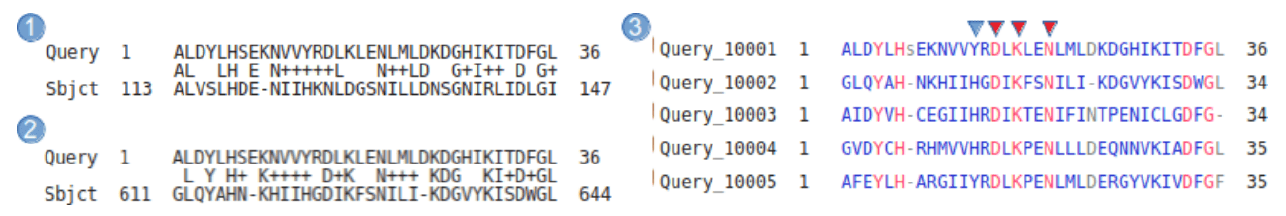
\includegraphics[width = \textwidth]{figs/msa.png}
\caption{\textbf{Pairwise vs MSA}. Se utilizó un fragmento del dominio quinasa de AKT7 humano (P31749) como consulta para buscar en una base de datos de proteínas archaca. (1) Alineación de AKTI y una ATPasa de la familia AAA (WP\_109940497.1) de \textit{Methanospirillum stamsii}. (2) Alineamiento del mismo fragmento de AKTI con una serina/treonina-proteína quinasa (OPY23844) de \textit{Methanobacterium sp}.. (3) MSA del sitio activo de 5 serina-treonina quinasas distantes. En flecha roja los residuos conservados en las 5 secuencias alineadas. Las puntas de flecha rojas marcan tres posiciones invariantes conservadas en todas las Ser/Thr-cinasas conocidas, el residuo Asp (D en esta tríada es el residuo del sitio activo. La punta de flecha azul marca una posición que está ocupada por His o Tyr en todas las proteínas conocidas de esta superfamilia).}
\label{fig:msa}
\end{figure}

\section{Métodos y esquemas de puntuación para la alineación de secuencias múltiples}
Como se explica en el capítulo anterior, la alineación óptima por pares puede lograrse eficazmente mediante algoritmos de programación dinámica. Estos métodos se basan en la construcción de una matriz $n \cdot m$, donde n y m corresponden a la longitud de las secuencias alineadas, y su complejidad en tiempo de ejecución es del orden de $O(n \cdot m)$ u $O(n^2)$ suponiendo que $n \sim m$. La extensión de este método a MSA es trivial. Por ejemplo, para tres secuencias de longitudes n, m y k, construiríamos una matriz $n \cdot m \cdot k$ que contenga las puntuaciones parciales óptimas para el alineamiento de tres posiciones. Sin embargo, la complejidad temporal en este caso sería de $O(n \cdot m \cdot k)$ u $O(n^3)$ suponiendo que $n \sim m \sim k$. De forma más general, para s secuencias de longitud n, la complejidad temporal sería $O(n^s)$ que crece exponencialmente con el número de secuencias. Por lo tanto, aunque este enfoque conduciría a un MSA óptimo, es poco práctico para más de unas pocas secuencias. Por este motivo, los métodos «simultáneos» no pueden aplicarse a problemas reales de MSA y se aproximan mediante métodos heurísticos que reducen el tiempo de cálculo pero no garantizan encontrar el alineamiento múltiple óptimo. Uno de los programas más populares para realizar MSA es ClustalW. Es un ejemplo de una familia de algoritmos que siguen una estrategia progresiva o jerárquica. Los métodos progresivos funcionan en tres pasos (véase la figura \ref{fig:clustalw}):
\begin{enumerate}
\item En el primer paso, este programa computa todos los posibles alineamientos por pares y calcula una puntuación bruta para cada alineamiento. La puntuación puede ser simplemente el porcentaje de identidades o medidas más sofisticadas.
\item A continuación, se realiza un análisis jerárquico de conglomerados en la tabla de puntuaciones por pares del paso anterior. Esta técnica produce un árbol guía o dendrograma que agrupa las secuencias según su similitud.
\item Por último, las secuencias se alinean progresivamente siguiendo la topología del árbol generado en el paso anterior. Así, se alinean las dos secuencias con la puntuación de similitud más alta y, a continuación, la secuencia siguiente se añade al alineamiento por pares o se utiliza en otro alineamiento por pares. Aunque no entraremos en detalles aquí, existen métodos rigurosos para alinear una secuencia contra un alineamiento. Imaginemos que la secuencia se alinea con una secuencia consenso derivada del alineamiento. El MSA puede representarse mediante estructuras matemáticas denominadas perfiles. En algún momento, los perfiles se alinean con los perfiles. Por último, el MSA se genera siguiendo el árbol guía desde los nodos más terminales hasta la raíz.
\end{enumerate}

\begin{figure}[htbp]
\centering
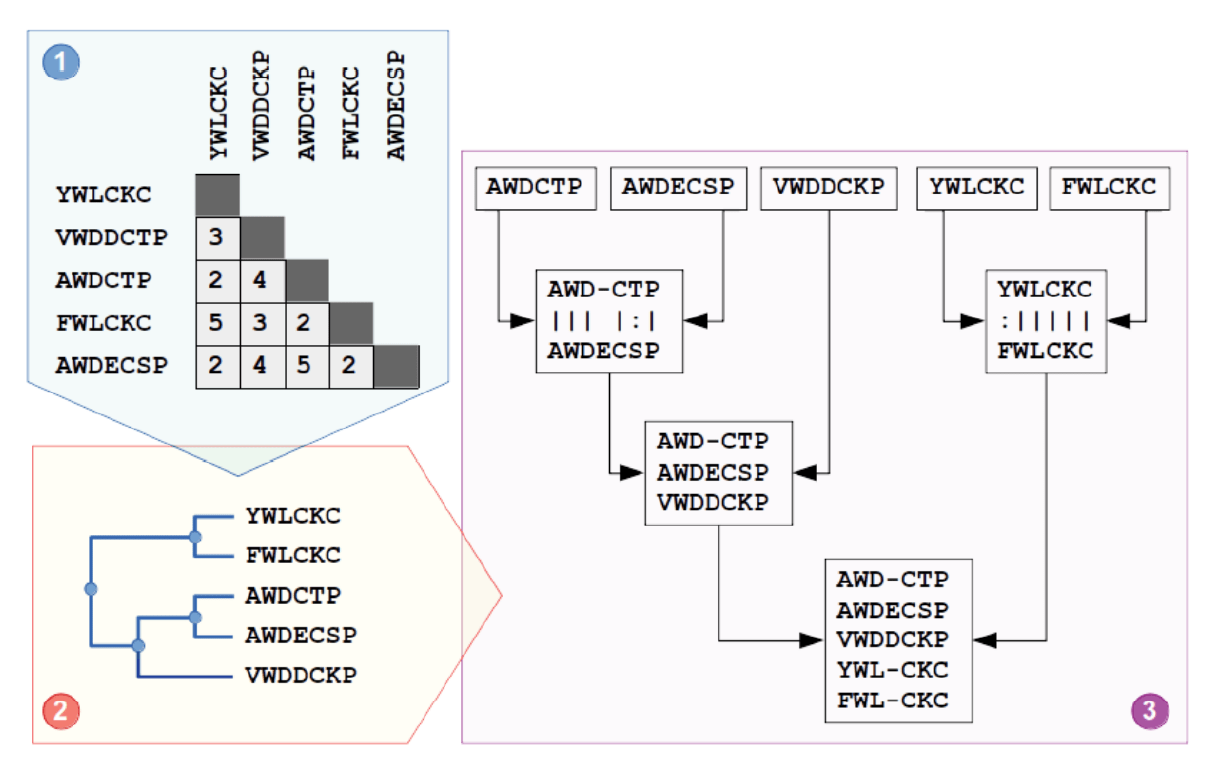
\includegraphics[width = \textwidth]{figs/clustalw.png}
\caption{\textbf{Métodos progresivos para el MSA}. Para producir un MSA de las secuencias YWLCKC (secuencia A), VWDDCTP (secuencia B). AWDCTP (secuencia C), FWLCKC (secuencia D) y AWDECSP (secuencia E), los métodos progresivos comparan primero todos los pares de secuencias (no mostrados) y registran la puntuación de cada alineamiento por pares (1). A continuación, basándose en estas puntuaciones, el algoritmo produce un árbol guía (2). Por último, las secuencias se alinean progresivamente empezando por las más cercanas. En cada paso del proceso, el algoritmo sigue la topología del árbol desde las hojas hasta la raíz, añadiendo nuevas secuencias o alineaciones en cada nodo del árbol (3).}
\label{fig:clustalw}
\end{figure}

Además de ClustalW, otras herramientas implementan variaciones de este algoritmo progresivo. Por ejemplo, ClustalW utiliza programación dinámica para el alineamiento por pares inicial, que es preciso pero puede ser lento para un gran número de secuencias. Por esta razón, otros métodos, como Kalign, cuentan el número de k-mers compartidos por las secuencias para calcular la distancia entre todos los pares. La ventaja de este método es que no es necesario alinear las secuencias para generar la matriz de distancias.

Uno de los problemas de los métodos progresivos es que el orden en que se añaden gradualmente las secuencias puede tener un fuerte impacto en el MSA final. Además, cuando se produce un error en un alineamiento intermedio, suele propagarse en los alineamientos posteriores. Esto es especialmente cierto en el caso de los gaps. Para mitigar estos problemas, diferentes algoritmos han adoptado variaciones en el procedimiento general, pero no las discutiremos aquí. Otro problema no resuelto en MSA es cómo calcular la puntuación. Se han propuesto varias estrategias:
\begin{itemize}
\item Scoring basado en una secuencia de referencia: $S_{MSA} = S_{AB} + S_{AC} + S_{AD} + S_{AE} $
\item Scoring basado en el dendograma: $S_{MSA} = S_{AB} + S_{CD} + S_{CD/E} + S_{AB/CDE}$
\item Scoring basado en la suma de alineamientos por pares: $S_{MSA} = S_{AB} + S_{AC} + S_{AD} + S_{AE} + S_{BC} + S_{BD} + S_{BE} + S_{CD} + S_{CE} + S_{DE}$
\end{itemize}

En resumen, aún no se ha resuelto el problema de calcular un MSA óptimo en un tiempo práctico. Mientras tanto, se han desarrollado varios enfoques heurísticos para calcular soluciones aproximadas que no garantizan ser la mejor solución posible.

Hasta ahora nos hemos centrado en el MSA de proteínas, sin embargo, el alineamiento múltiple de secuencias de regiones genómicas merece especial atención debido a la creciente cantidad de genomas completos disponibles y a su relevancia para identificar regiones genómicas reguladoras y comprender la variabilidad genética interindividual e interespecífica. Aunque no entraremos en detalles, la alineación de regiones genómicas plantea retos específicos. Por ejemplo, los genomas contienen un gran número de regiones repetitivas que son difíciles de alinear con precisión. Además, aunque la secuencia de determinadas regiones del genoma pueda conservarse en diferentes especies, a menudo la posición relativa de las distintas porciones del genoma no se conserva debido a reordenamientos genómicos. Por último, los MSA proteínicos suelen estar formados por un gran número de secuencias relativamente cortas, mientras que ocurre lo contrario con los MSA genómicos. Por todas estas razones, la alineación genómica requiere métodos de MSA especializados. Uno de ellos es MLAGAN, que se basa en un método progresivo similar al utilizado por ClustalW, y MULTIZ, utilizado para producir el MSA genómico que muestra el navegador del genoma de la UCSC.

\subsection{Ejemplo: FOXP2}
FOXP2 es un factor de transcripción. Al realizar un alineamiento de múltiples secuencias, se observan algunos residuos que presentan unos cambios únicos en humanos y son los que nos aportan la capacidad de comunicación como el habla. Además, individuos que tienen mutados esos individuos presentan un desorden del lenguaje. Por tanto, esos residuos son clave, y esto se demostró en ratones a los que se les cambió esos residuos concretos. Visto que esos cambios aparecen específicamente en humanos y que introducidos en ratones producen un comportamiento similar al habla, se analizó la filogenia y se observó exclusivamente en \textit{Homo sapiens} y Neandertales, pero no en otros primates.

\begin{figure}[htbp]
\centering
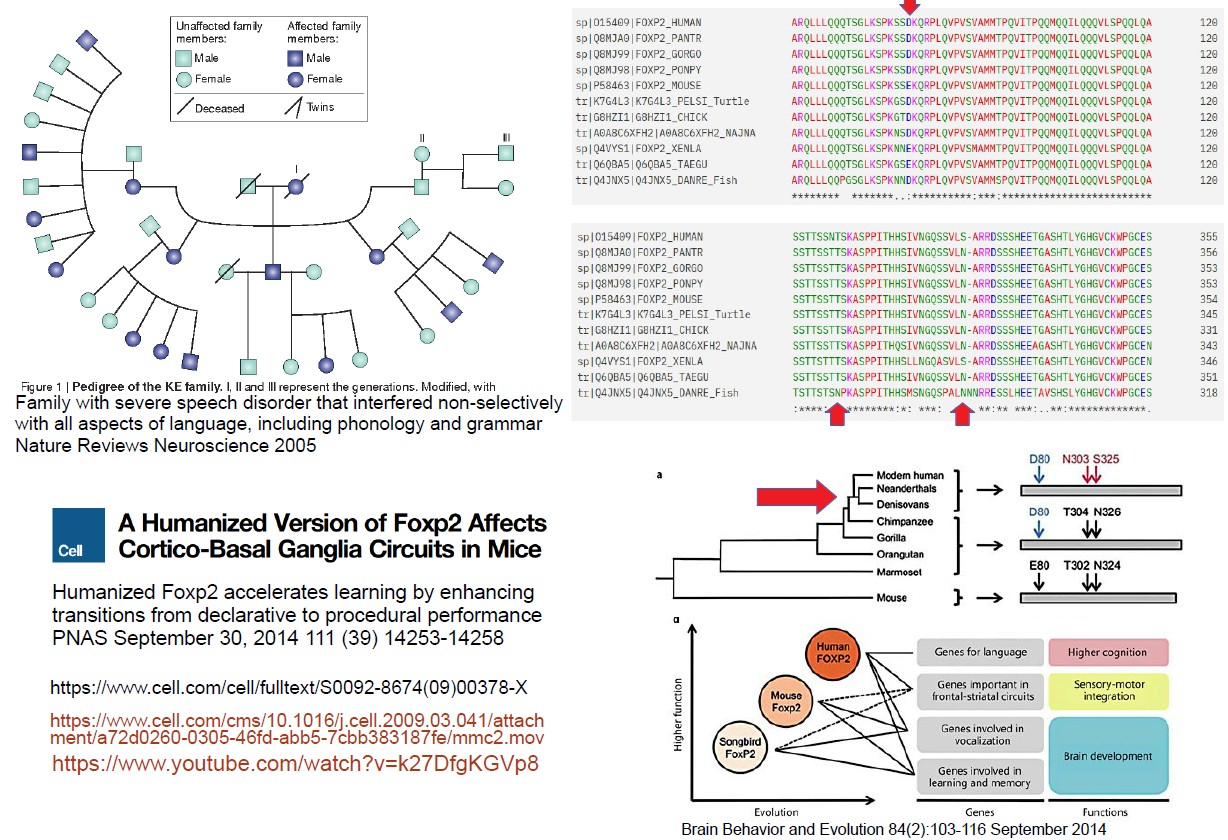
\includegraphics[width = \textwidth]{figs/foxp2.png}
\caption{Ejemplo del factor de transcripción FOXP2}
\end{figure}

%14/10 - Luis del Peso
\section{Representación de MSA}
Como se ha explicado anteriormente, el MSA puede utilizarse para identificar motivos/dominios funcionales y/o estructurales en un grupo de secuencias. Y lo que es más importante, una vez que hemos identificado ese motivo/dominio, puede utilizarse para buscar en bases de datos e identificar otras proteínas que compartan ese (nuevo) motivo y, como veremos, esas búsquedas son mucho más sensibles que las basadas en una secuencia de consulta. Sin embargo, para realizar dichas búsquedas, necesitamos una forma de representar el motivo/dominio revelado en el MSA. Existen varias formas de representar una región conservada, como se explica a continuación.

\subsection{Secuencia consenso}
Esta es la forma más sencilla de representar una región conservada y se utiliza ampliamente debido a su simplicidad y a su interpretación directa. Para construir una secuencia de consenso podríamos limitarnos a representar aquellos residuos que se conservan en todas las secuencias en una posición determinada. Por ejemplo, la secuencia consenso para la MSA representada en la figura \ref{fig:consensus-seq} es: TTxCxxAAxx donde x representa cualquier aminoácido. De hecho, esto se denomina consenso al 100\% de frecuencia, porque un residuo sólo se incluye en el consenso cuando está presente en el 100\% de las secuencias alineadas. El consenso puede construirse a cualquier otro nivel de porcentaje. Para el mismo alineamiento, el consenso al 50\%, que representa residuos presentes en al menos el 50\% de las secuencias, sería TTGCTCAAXT. Por último, a menudo el consenso representa el residuo más frecuente en cada posición, independientemente de su frecuencia absoluta.

\begin{figure}[htbp]
\centering
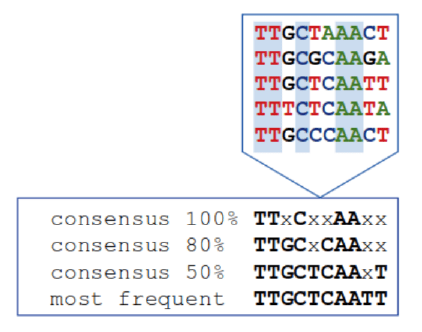
\includegraphics[width = 0.5\textwidth]{figs/consensus-seq.png}
\caption{\textbf{Secuencia consenso.} La secuencia de consenso indica el residuo presente en al menos un determinado porcentaje de las secuencias alineadas, o simplemente el residuo más frecuente, en cada posición del MSA. La figura muestra la alineación de varias secuencias de ADN unidas por C/EBP.}
\label{fig:consensus-seq}
\end{figure}

\subsection{Expresiones regulares o patrones}
El problema de las secuencias de consenso es que se pierde la mayor parte de la información contenida en el alineamiento. Por ejemplo, el consenso TTxCxxAAxx implica que no hay preferencia de residuo en la tercera posición. Sin embargo, la inspección de las secuencias individuales revela que, de hecho, existe una fuerte preferencia por la guanina en esta posición.
Por otra parte, el consenso del 50\% capta la preferencia por G en esta posición, pero no informa sobre qué otros residuos (si los hay) pueden ocupar esta posición ni sobre su frecuencia. Esta deficiencia es evidente en la décima posición del consenso del 50\%, que no muestra que en esta posición son posibles tanto la timina como la adenina. Las \textbf{expresiones regulares}, también conocidas como \textbf{patrones}, utilizan un conjunto de reglas para capturar esta diversidad. Por ejemplo, representan todos los residuos alternativos posibles en una posición determinada entre corchetes. También se puede representar aquellos residuos que nunca aparecen entre llaves. Así, el MSA de la figura \ref{fig:consensus-seq} puede representarse mediante la expresión regular:\\
TT[GT]C[TGC][AC]AA[TGC][TA]\\
TT[GT]C\{A\}[AC]AA\{A\}[TA]\\
Esta representación proporciona más información que las contras correspondientes, ya que muestra que la décima posición puede estar ocupada por T o A.

\subsection{Matrices de puntuación específicas para cada puesto (PSSM)}
Aunque las expresiones regulares representan una mejora con respecto al consenso, pierden importante información orientativa. La expresión regular mostrada en la sección anterior indica que T, C o G pueden encontrarse en las posiciones quinta y novena. Sin embargo, la preferencia por la timina es mayor en la quinta posición (0,6 frente a 0,4 de frecuencia). Una estructura que captura este tipo de información cuantitativa es la Matriz de Puntuación de Posiciones Específicas (PSSM). Una PSSM no es más que una matriz que confronta todos los símbolos posibles (los 20 aminoácidos posibles o los 4 nucleótidos en las secuencias de nucleótidos) con las posiciones de alineación. Cada celda de la matriz contiene un número que representa la preferencia de cada residuo concreto en cada posición. Hasta ahí, se consideraría una PWM (position weight matrix), es decir, tomar las frecuencias de cada nucleótido para cada posición normalizadas. Formalmente, los valores de cada celda de la PSSM se calculan como la relación logarítmica entre las frecuencias de residuos observadas en cada posición y las esperadas por azar. Así, suponiendo frecuencias de fondo iguales para todos los nucleótidos, el PSSM que representa el MSA mostrado en \ref{fig:consensus-seq} sería:

\begin{table}[htbp]
\centering
\begin{tabular}{l | l l l l l l l l l l }
& 1 & 2 & 3 & 4 & 5 & 6 & 7 & 8 & 9 & 10 \\ \hline
A & -1,2 & -1,2 & -1,2 & -1,2 & -1,2 & 0 & 1,4 & 1,4 & -1,2 & 0,4 \\
C & -1,2 & -1,2 & -1,2 & 1,4 & -0,2 & 1,2 & 1,2 & 1,2 & 0,4 & -1,2  \\
G & -1,2 & -1,2 & 1,2 & -1,2 & -0,2 & -1,2 & -1,2 & -1,2 & -0,2 & -1,2  \\
T & 1,4 & 1,4 & -0,2 & -1,2 & 0,8 & -1,2 & -1,2 & -1,2 & 0,4 & 0,8  \\
\end{tabular}
\caption{PSSM representando el MSA de la figura \ref{fig:consensus-seq}}
\end{table}

Por ejemplo, la entrada correspondiente a la timina en la posición 1 se calcularía como $log_2 \frac{5/5}{0,25} = 1,4$. Sin embargo, como $log_2(0)$ no está definido, esta ecuación produciría un error si se aplicara a la entrada de A en la primera posición $(log_2(\frac{0/5}{0,25}))$. Para evitar este problema utilizamos \textbf{pseudoconteos}, es decir, añadimos un pequeño valor, $\beta$, a cada celda para que la frecuencia observada nunca sea cero. Así, si la frecuencia observada del símbolo $i$ en la posición $p, f_{ip}$ es $n_{ip}/N_{seq}$, donde $n_{i,p}$ es el número de residuos del tipo $i$ alineados en la columna $p$ y $N_{seq}$ es el número de secuencias alineadas, entonces la frecuencia de $i$ después de añadir pseudoconteos sería:
$$f_{i,p} = \frac{n_{i,p} + \beta}{N_{seq} + (\beta \cdot N_s)}$$

donde $N_s$ es el número de los diferentes símbolos (4 en el caso de los nucleótidos y 20 para proteínas). Obsérvese que, de hecho, esta corrección es una forma de superar la falta de datos a la hora de derivar los valores de un PSSM. Por ejemplo, en el caso de la figura \ref{fig:consensus-seq}, ¿hasta qué punto estamos seguros de que la adenina nunca se encuentra en la posición 1? Si en lugar de sólo cinco instancias de C/EBP tuviéramos 500, ¿tendrían algunas de ellas «A» en la primera columna? El valor de $\beta$ suele ser 1 para la construcción de PSSMs, lo que implica que observaríamos al menos un residuo de cada tipo en cada columna si tuviéramos datos suficientes, pero podríamos elegir cualquier otro valor. Tras aplicar pseudoconteos la entrada correspondiente a la timina en la posición 1 se calcularía como $log _2(\frac{6/9}{0,25}) = 1,41$ y la entrada de A en la primera posición sería $log_2(\frac{1/9}{0,25}) =-1,2$.

El problema de este modelo es que asume la independencia entre posiciones, cuando esto es falso. Además, no se pueden representar fácilmente los gaps, solo se podría apañar haciendo una PSSM antes del gap y otra después.

\subsubsection{Generación de PSSM: un caso real}
En el siguiente ejemplo se oberva la frecuencia de nucleótidos en el motivo TATA derivado de más de 800 secuencias de promotores de mamíferos de GenBank que tenían anotados un motivo TATA.

\begin{figure}[htbp]
\centering
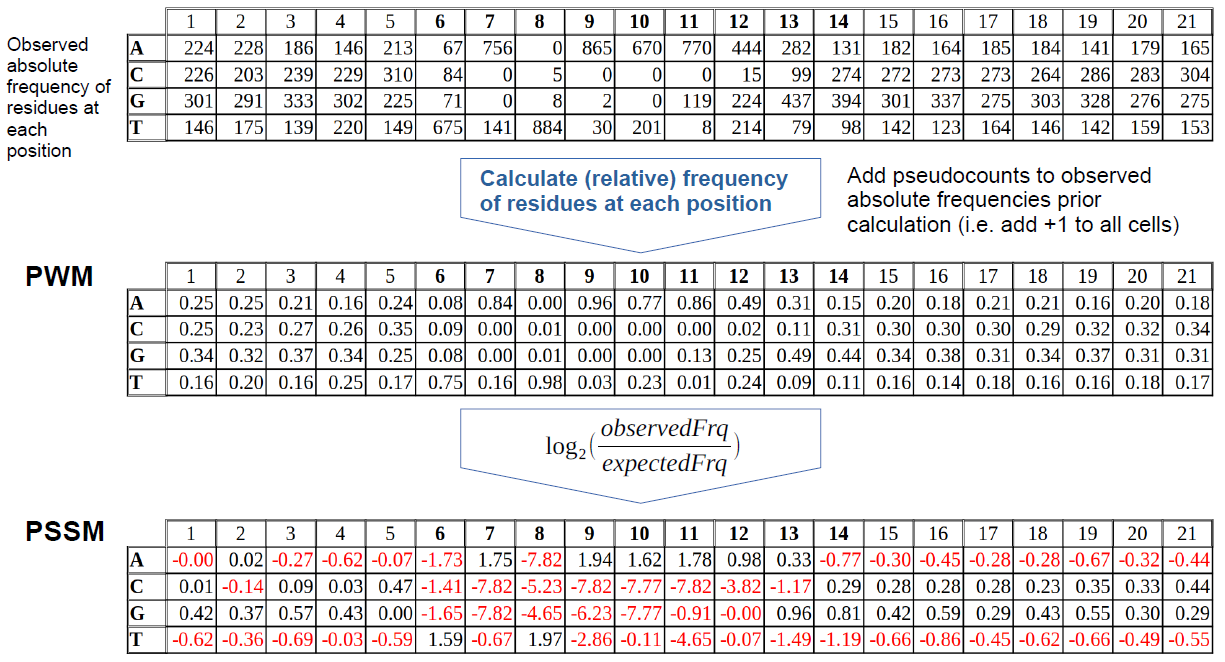
\includegraphics[width = \textwidth]{figs/tata.png}
\caption{Frecuencia de nucleótidos en el motivo TATA derivada de >800 secuencias promotoras de mamíferos de GenBank que tenían elementos TATA anotados a $\sim$ -30 pb del TSS.}
\end{figure}

\subsection{Secuencia de logotipos y contenido informativo}
Los PSSM y los HMM son formas precisas de representar la MSA. Son especialmente fáciles de manipular por ordenador y, por tanto, aptos para representar motivos y dominios proteicos en bases de datos especializadas y para buscar en bases de datos. Sin embargo, no son una forma fácil de representar MSA para el ser humano.

Por este motivo, en publicaciones y libros, los patrones de un conjunto de secuencias alineadas se suelen mostrar mediante una representación gráfica denominada \textbf{logo}. En un logo, los símbolos encontrados en cada posición del alineamiento se muestran apilados unos sobre otros, ordenados según su frecuencia (el símbolo más frecuente se muestra encima del resto). Además, la altura de los símbolos es proporcional a su frecuencia, de modo que se resaltan los símbolos preferidos en cada posición. Por último, la altura total de cada columna de símbolos se ajusta para significar la conservación global de los símbolos. Así, las posiciones que muestren una fuerte preferencia por un determinado tipo de residuos serán altas, mientras que las posiciones que muestren poca conservación estarán representadas por una pila corta de símbolos. La representación resultante revela claramente el patrón que definen las secuencias alineadas (véase la figura \ref{fig:logo}).

\begin{figure}[htbp]
\centering
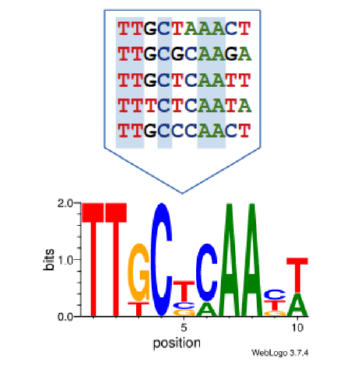
\includegraphics[width = 0.3\textwidth]{figs/logo.png}
\caption{\textbf{Logo}. Representación de la alineación mostrada en la figura \ref{fig:consensus-seq} como logo. El gráfico se generó con WebLogo3 sin ajustes de composición y utilizando un esquema de colores clásico.}
\label{fig:logo}
\end{figure}

Los logos de secuencias se basan en el concepto de entropía de la teoría de la información, desarrollado por Claude Shannon. El grado de conservación de los residuos en una posición concreta de un MSA puede cuantificarse, utilizando las herramientas de la teoría de la información, como la cantidad de incertidumbre sobre los posibles residuos que pueden ocupar esa posición. Por ejemplo, dado el MSA representado en la figura \ref{fig:logo}, nuestra incertidumbre sobre el nucleótido que puede encontrarse en la posición 1 de un sitio de unión a C/EBP es muy pequeña. Así, si alguien encuentra una nueva región unida por C/EBP será fácil predecir el nucleótido presente en la primera posición antes de ver este nuevo sitio de unión. En cambio, sería mucho más difícil predecir con certeza la identidad del residuo en la novena posición. En el campo de la información, la entropía \footnote{Formalmente, se llama entropía de Shannon}, H, de una variable aleatoria discreta X con valores posibles $x_1, x_2, \ldots ,x_n$ es una medida de la cantidad de incertidumbre asociada al valor de X (cuantifica la información). La entropía de Shannon se define como:
$$H(X) = -\sum_i P((x_i) log_2 P(x_i)$$
donde $P(x_i)$ es la probabilidad de observar el valor $i$-ésimo de X. La entropía, $H(X)$, se mide en unidades de bits. El término bit (que no byte) es una acortación de "binary digit" y representa la unidad básica de información en comunicación computacional y digital. En ese sentido, el término $P(x_i) log_2 P(x_i)$ es 0 cuando $P(x_i) = 0$.

Podemos pensar en los bits como el número mínimo de dígitos binarios necesarios para representar todos los estados de un sistema. Por ejemplo, el lanzamiento de una moneda puede dar dos resultados (estados): cara o cruz. Un solo dígito binario puede representar ambos (0 o 1). Por tanto, la entropía asociada al lanzamiento de una moneda es: $-(P_{head} log_2 P_{head} + P_{tail} log_2 P_{tail}) = 1 bit$. 
Del mismo modo, lanzar un dado puede dar lugar a 6 estados diferentes, por lo que para representar todos los casos posibles necesitaríamos tres dígitos binarios. Nótese que, en este caso, tres dígitos binarios es un exceso, ya que pueden representar hasta 8 estados (000, 001, 010, 100, 011, 101, 110, 111), mientras que nosotros sólo necesitamos representar 6. Sin embargo, dos dígitos binarios serían insuficientes para representar los seis estados. Por eso la entropía asociada es de 2,6 bits en lugar de 3. Último ejemplo: la incertidumbre de que haya un nucleótido en una cierta posición es:
\begin{align*}
H(nucleotide) = - \sum_{x_i = A, C, G, T} P(x_i) log_2 P(x_i) = \\
 - ((\frac{1}{4} \cdot log_2\frac{1}{4}) + (\frac{1}{4} \cdot log_2\frac{1}{4}) + (\frac{1}{4} \cdot log_2\frac{1}{4}) + (\frac{1}{4} \cdot log_2\frac{1}{4})) = 2 bits
\end{align*}
Por tanto, el genoma humano puede almacenar una capacidad máxima de información de:
$$3,2 \cdot 10^9 pb \cdot 2 bits = 6,4 \cdot 10^9 bits = 800 Mb = 0,8 Gb$$
Solo se tiene en cuenta una cadena y no las dos ya que, al ser complementarias, la información codificada es la misma en ambas cadenas y, por tanto, redundante. 
Bajo los estándares actuales, esta cantidad de información es ridícula. En el ADN está toda la información necesaria para hacer cualquier individuo completo. No obstante, el genoma codificante es un 1-2\%. Esto es crítico, ya que se genera mucha complejidad con tan poca información. El tema está en que nuestro genoma no codifica la información de cada neurona, solo codifica proteínas, las cuales interaccionan entre sí y generan propiedades emergentes. Así, hay una capa superpuesta de información que no es evidente y explica toda la complejidad. 
Nuestro genoma acumula muy poca información, pero es muy pequeño. Por unidad de volumen, la densidad de información a guardar es mucho más grande. Otra ventaja fundamental es que el ADN es muy estable, incluso almacenado de forma no óptima. Por ejemplo, los fósiles siguen teniendo ADN que se puede recuperar; no se puede decir lo mismo de un teléfono móvil 3 semanas a la intemperie. Por ello, se está intentando almacenar información en el ADN, pero el problema es cómo guardarlo y recuperarlo, ya que depende de procesos bioquímicos sensibles.

Volviendo a los logos, la altura de cada columna de símbolos representa el contenido informativo de esa posición concreta. Debemos pensar en el contenido informativo como una disminución de la incertidumbre tras la recepción de algún mensaje o dato. Así, el contenido informativo o entropía relativa es la diferencia entre la entropía (es decir, la incertidumbre) antes y después del mensaje:
$$I(X) = H_b(X) - H_a(X)$$
donde $I(X)$ es la información, $H_b$ la incertidumbre inicial y $H_a$ la entropía después de haber recibido algunos datos.
Por ejemplo, la incertidumbre sobre el resultado de tirar un dado antes de lanzarlo es de 2,6 bits. Si alguien tira los dados (sin que veamos el resultado) y nos informa de que el resultado ha sido un número par, entonces la entropía tras recibir este nuevo dato es de 1,6 bits. Así, podemos cuantificar la información recibida como $H_{before} - H_{after}$ correspondiente a 1 bit. En el caso de las secuencias biológicas, ver el MSA reduce nuestra incertidumbre sobre el símbolo esperado en cada posición y esta reducción se cuantifica por el contenido de información de cada posición. Nótese que hemos estado calculando el contenido de información para posiciones individuales. La ganancia total de información se obtiene sumando todas las posiciones. Al hacerlo, partimos del supuesto simplificador de que las frecuencias de una posición no se ven influidas por las de otra posición. Así, el contenido total de información para el MSA se calcula como:
$$I = \sum_i H_i^b - H_i^a$$
donde $i$ representa cada posición en el alineamiento.

\begin{table}[htbp]
\begin{mdframed}[backgroundcolor=black!10]
En resumen, los logos son representaciones de los alineamientos donde se representan los nucleótidos en cada posición, siendo el tamaño del nucleótido representativo de su frecuencia. En este caso, el eje y muestra bits, que son una unidad de información. Cuantas más posibilidades (outcome, $x_i$) hay, más incertidumbre hay y, por tanto, mayor es la entropía de Shannon. 

Algunas posiciones llegan a los 2 bits, es decir, almacenan toda la información que es posible almacenar. Sin embargo, hay otras posiciones que son menores que 2 bits. Esto se debe a que no se muestra la entropía, si no la información: la incertidumbre de un proceso antes y después de recibir información adicional. Antes de un alineamiento, la incertidumbre en cada posición es de 2 bits. Si tras hacer el alineamiento una posición tiene siempre un mismo nucleótido, la incertidumbre pasa a ser 0, por lo que la información es 2 - 0 = 2. Cuanto más variable sea una posición en el alineamiento, más incertidumbre hay y menos información tenemos. En los logos, la altura es el contenido de información y el tamaño de cada letra es la probabilidad de que salga.
\end{mdframed}
\end{table}

\begin{figure}[htbp]
\centering
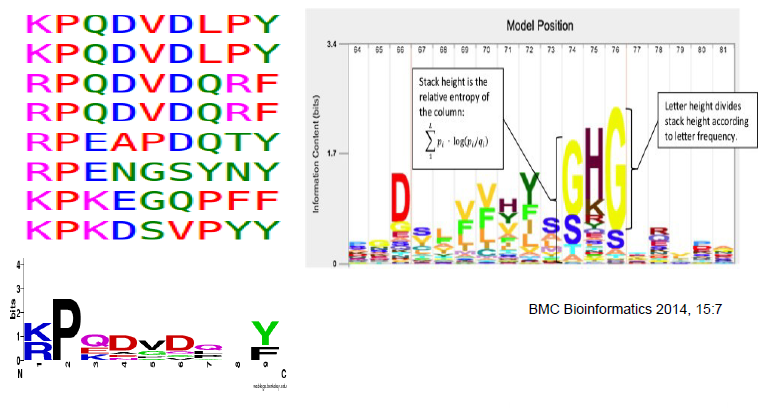
\includegraphics[width = \textwidth]{figs/logo-parts.png}
\caption{Partes de un logo.}
\end{figure}

%\subsection{Modelos de Markov ocultos (HMM)}

\chapter{Preguntas adicionales}
\section{Examen de prueba: Autoevaluación del curso}
\subsection{Exercise 1}
We have a sequence 5241977 bases long. Table below shows the sequence statistics.

\begin{table}[htbp]
\centering
\begin{tabular}{l | l l l l l }
& overall & from A & from C & from G & from T \\ \hline
to A & 0.247 & 0.296 & 0.277 & 0.229 & 0.187 \\
to C & 0.253 & 0.223 & 0.231 & 0.323 & 0.235 \\
to G & 0.252 & 0.208 & 0.289 & 0.230 & 0.281 \\
to T & 0.247 & 0.273 & 0.202 & 0.218 & 0.298
\end{tabular}
\end{table}

How many TATA-box motifs (TATAAT) would you expect by chance according to a simple multinomial model?
$$ 0.247^6 \cdot 5241977 = 1190.36 \approx 1190 $$

And according to a Markov-chain model where the initial prob. is the same as overall one?
$$0.247 \cdot 0.187 \cdot 0.273 \cdot 0.187 \cdot 0.296 \cdot 0.273 \cdot 5241977 = 998.83 \approx 999 $$

\subsection{Exercise 2}
The following contains a python function that accepts a DNA sequence and returns the data structure AbsdiNucl\_freq containing the absolute frequencies of dinucleotides. 

\begin{lstlisting}
## Function to count absolute dinucleotide frequencies
def AbsdiNuclFrq(Seq):
	# Initializes a dictionary for all 16 potential dinucleotides
	AbsdiNucl_freq = {}
	for Base1 in ["A", "C", "G", "T"]:
		for Base2 in ["A", "C", "G", "T"]:
			AbsdiNucl_freq[Base1+Base2] = 0
	# count frequencies
	for pos in range(0, len(Seq) - 1):
		if Seq[pos:pos+2] in AbsdiNucl_freq.keys():
			AbsdiNucl_freq[Seq[pos:pos+2]] = AbsdiNucl_freq[Seq[pos:pos+2]]+1
	# Sequence length
	return(AbsdiNucl_freq) #return a identifier-null dict.
\end{lstlisting}

Which of the following expressions would you use to retrieve the frequency of the dinucleotide GC? \textbf{Since the frequencies are stored in a dictionary, we can just index by the dinucleotide we are interested in, so: AbsdiNucl\_freq["GC"]}

\subsection{Exercise 3}
The following figure shows several Dot-Matrix obtained from the alignment of different combinations of the indicated protein sequences or the indicated DNA sequences. Indicate which sequences were aligned in each case.
\begin{figure}[htbp]
\centering
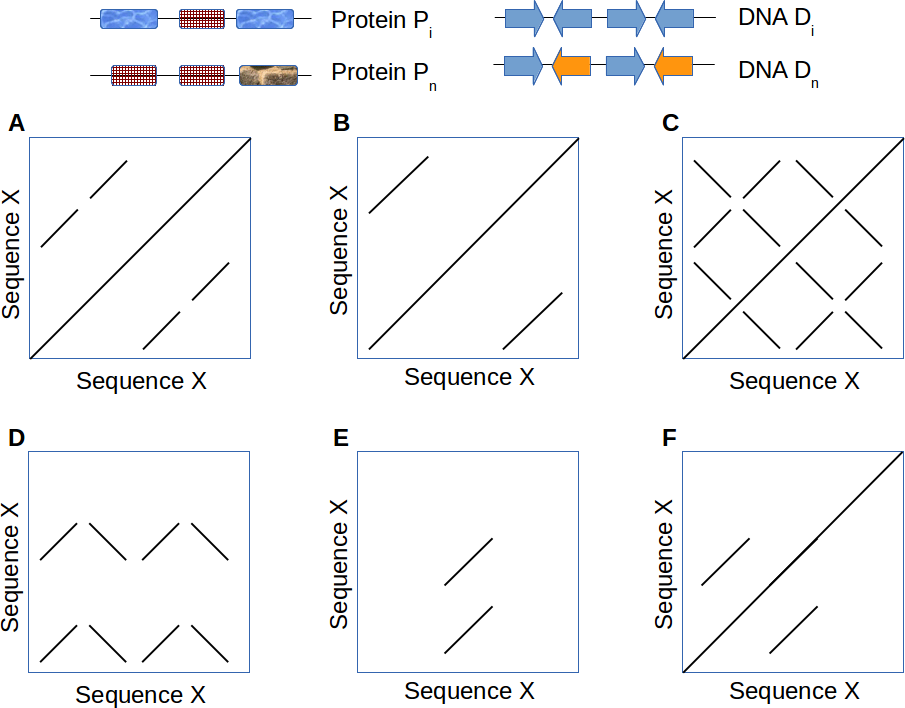
\includegraphics[width = 0.7\textwidth]{figs/exam-ex3.png}
\end{figure}

Trick: when a sequence is aligned with itself, there is a whole diagonal in the dot matrix.

\noindent
Dot-Matrix A: DNA Dn vs DNA Dn \\
Dot-Matrix B: Protein Pi vs Protein Pi \\
Dot-Matrix C: DNA Di vs DNA Di\\
Dot-Matrix D: DNA Di vs DNA Dn \\
Dot-Matrix E: Protein Pi vs Protein Pn \\
Dot-Matrix F: Protein Pn vs Protein Pn \\

\subsection{Exercise 4}
Indicate the optimal method to apply in the following situations:
\begin{enumerate}
\item Protein search against a database to identify similar proteins: \textbf{BLAST}
\item  You are interested in finding conserved domains within a set of given sequences: \textbf{Smith-Waterman - local alignment}
\item You need the best alignment between the whole extension of two proteins: \textbf{Needleman-Wunsch - global alignment}
\item Quick identification of repeated sequences between two chromosomes: \textbf{Dot-Matrix}
\end{enumerate}

\subsection{Exercise 5}
We performed a pairwise alignment between the human HRAS and the indicated \textit{C. elegans} proteins using BLAST(p) with default parameters and got the indicated scores. The figure shows the probability density (graphs on top) and cumulative probability (bottom graphs) for the BLAST score values for random alignments under these conditions (graphs on the right are just a zoom of the left graphs on the values 30 to 90). The red lines mark the position of problem scores. Indicate the probability of getting an alignment with an associated score equal or higher than these just by chance (choose the one that best describes it):

\begin{figure}[htbp]
\centering
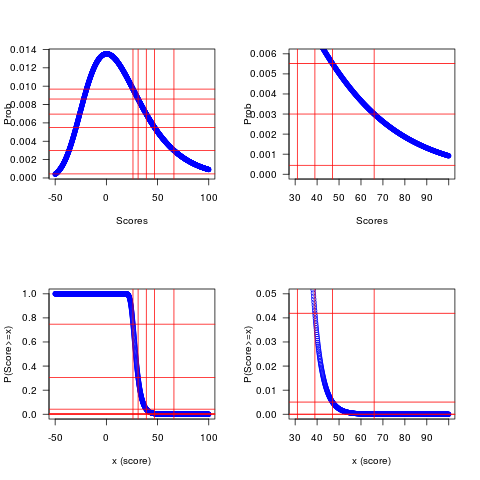
\includegraphics[width = 0.7\textwidth]{figs/exam-ex5.png}
\end{figure}

For this problem we have to use the cumulative probabilities (bottom graphs):
\begin{enumerate}
\item  KBRAS, score=120. p-value: \textbf{<0.001}
\item ARL2, score=66. p-value: \textbf{<0.001}
\item CKI1, score=47. p-value: \textbf{<0.01}
\item MED20, score=39. p-value: \textbf{<0.05}
\item ZK688, score=31. p-value: \textbf{>0.05}
\item RL15, score=26. p-value: \textbf{>0.05}
\end{enumerate}

\subsection{Exercise 6}
To generate the alignment between two sequences (of length m and n) using dynamic programing we follow these steps:
\begin{enumerate}
\item  Fill a m*n matrix with the scores resuting from: 
$$ Score = Max 
  \begin{cases}
    F(i-1, j-1) + s(x,y)\\ 
    F(i-1, j) - GapPenalty \\
    F(i, j-1) - GapPenalty
  \end{cases}
$$
  
\item  Reconstruct the alignment. Starting from bottom-right cell of the matrix generated in \#1 trace-back the pointers to the initial top-left cell.
\end{enumerate}

The pseudocode for this algorithm is depicted here:
\begin{figure}[htbp]
\centering
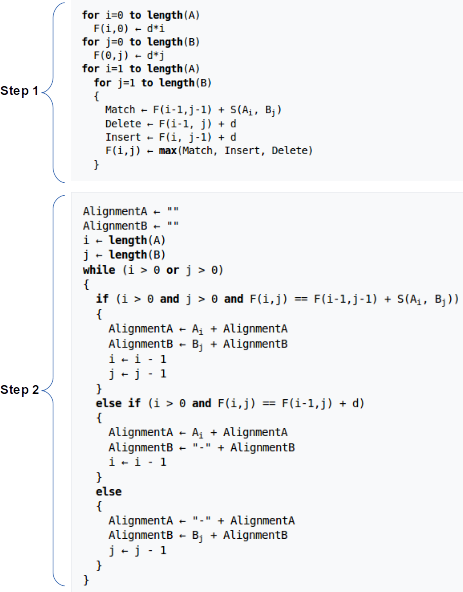
\includegraphics[width = 0.5\textwidth]{figs/exam-ex6.png}
\end{figure}

Are the pointers saved during the generation of the matrix (step 1)? \textbf{NO}

\subsection{Exercise 7}
Big-O notation is used to: \textbf{describe concisely the running time of an algorithm.}

\subsection{Exercise 8}
Match the following MSA with the simplest model that preserves most of the information in that alignment. keeping in mind that you can choose each model only once.
\begin{figure}[htbp]
\centering
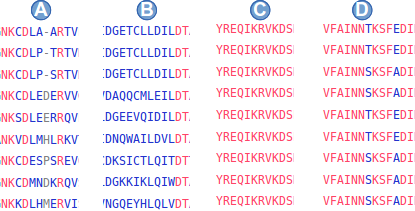
\includegraphics[width = 0.7\textwidth]{figs/exam-ex8.png}
\end{figure}

\noindent
Alignment A: \textbf{Hidden Markov Model (HMM)} \\
Alignment B: \textbf{Position Specific Scoring Matrix (profile) (PSSM)} \\
Alignment C: \textbf{Consensus sequence} \\
Alignment D: \textbf{Regular expression (pattern)}

Los modelos ordenados por orden de complejidad ascendente son secuencia consenso, patrón, PSSM y HMM. Con eso, solo es cuestión de ordenar los alineamientos por complejidad y asignar el modelo.

\subsection{Exercise 9}
We have aligned several tyrosine protein kinases and found a conserved region corresponding to the active site of these enzymes. Here is the regular expression representing this alignment: [LIVMFYC]-{A}-[HY]-x-D-[LIVMFY]-[RSTAC]-{D}-{PF}-N-[LIVMFYC] 

\begin{figure}[htbp]
\centering
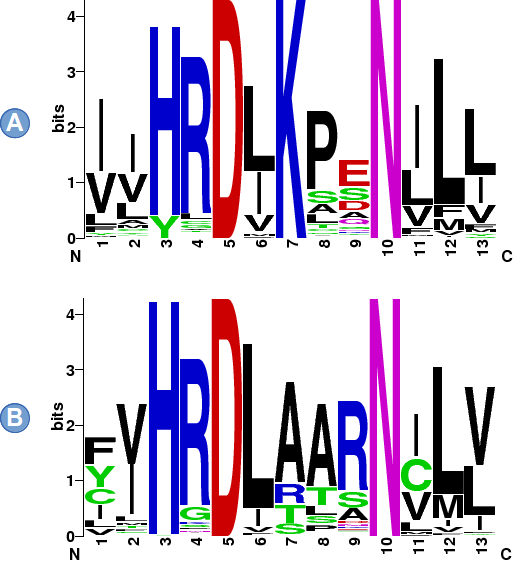
\includegraphics[width = 0.4\textwidth]{figs/exam-ex9.png}
\end{figure}

Which of the sequence logos in the figure represent this alignment? \textbf{B} \\
Which of the following positions shows the lowest information content in that alignment? \textbf{Position 1}

\subsection{Exercise 10}
Commonly used MSA programs: \textbf{use an heuristic approach composed of three steps: distance calculation, dendrogram tree generation, pairwise alignment based on tree topology.}

BLAST uses  an heuristic approach composed of three steps (construction of a word list from the sequences, identification of identical words (seeds), extension of seeds) for the search of a sequence within a database. 

Global and local alignments between two sequences  use an extension of dynamic programming to generate the alignment.

\section{Preguntas anteriores}
\subsection{Exercise 1}
You have access to a fragment of the genome of a new ssDNA virus. We assume it is a representative fragment and that the composition is homogeneous throughout the genome. The frequencies of bases in this sequence fragment are given in the table below. Use Maximum Likelihood (ML) to estimate the following parameters of a basic multinomial model and a Markov-chain model for this sequence:

Multinomial model, probability of A, $P_A = \frac{1}{4} = 0,25 $

\begin{table}[htbp]
\centering
\begin{tabular}{l | l l l l }
& from A & from C & from G & from T \\ \hline
To A & 21 & 37 & 41 & 25 \\
To C & 21 & 62 & 58 & 17 \\
To G & 35 & 50 & 26 & 27 \\
To T & 47 & 11 & 13 & 9
\end{tabular}
\end{table}

Markov-model probability of transition from T to A, $P_{TA} = \frac{from T to A}{from T to everything} = \frac{25}{25 + 17 + 27 + 9} = 0.3205$

\subsection{Exercise 10}
According to data in the figure, the observed mutation frequency Met/Arg is the same as Phe/Asn. What about their corresponding entries in the BLOSUM62 substitution matrix?

\begin{figure}[htbp]
\centering
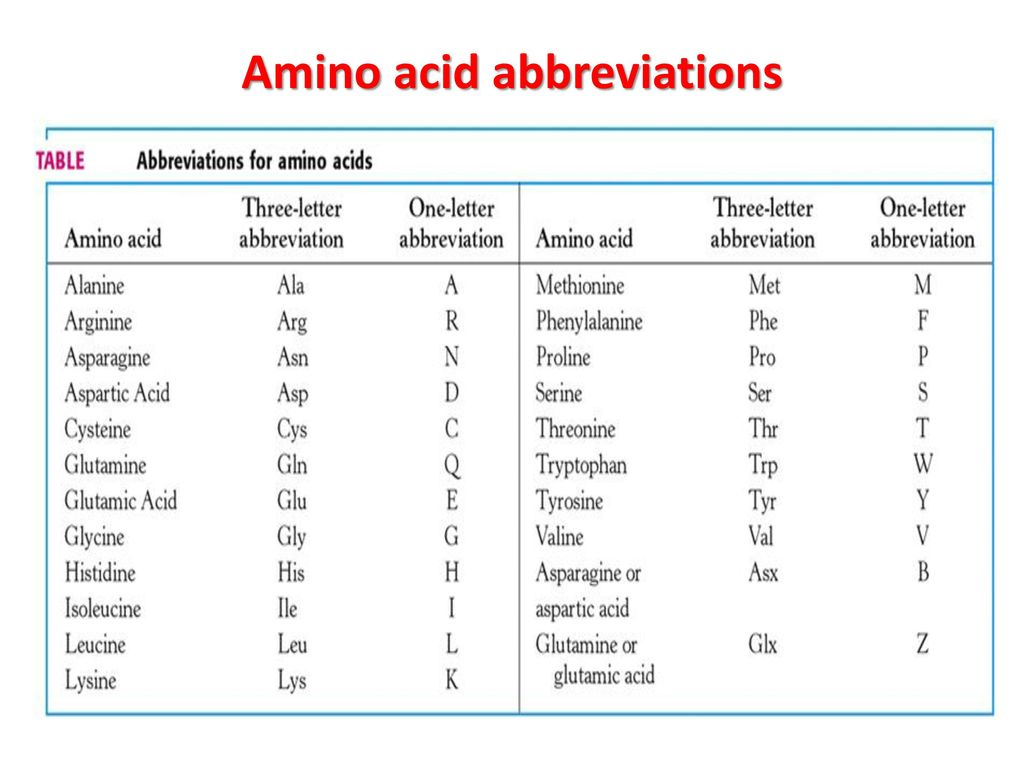
\includegraphics[width = 0.7\textwidth]{figs/aa_abbreviations.png}
\end{figure}

The observed mutation frequency is 8/1000. For the entry in the BLOSUM62 substitution matrix ($2 \cdot log_2 (odds ratio) = 2 \cdot log_2 (\frac{observed}{expected}$):
$$S_{M, R} = 2 \cdot log_2 (\frac{8/1000}{0.025 \cdot 0.052}) = 5.243$$
$$S_{F, N} = 2 \cdot log_2 (\frac{8/1000}{0.047 \cdot 0.045}) = 3.839$$
In conclusion, \textbf{Met/Arg have higher entry value than Phe/Asn}.

If all the entries in the diagonal of the mutation frequency table were the same, what would be their corresponding entry in the scoring matrix? \textbf{If the observed value would be the same for the entire diagonal, their values for the scoring matrix would be determined by their expected values. W has the lowest expected value and would therefore have the highest value in the scoring matrix.}

\begin{figure}[htbp]
\centering
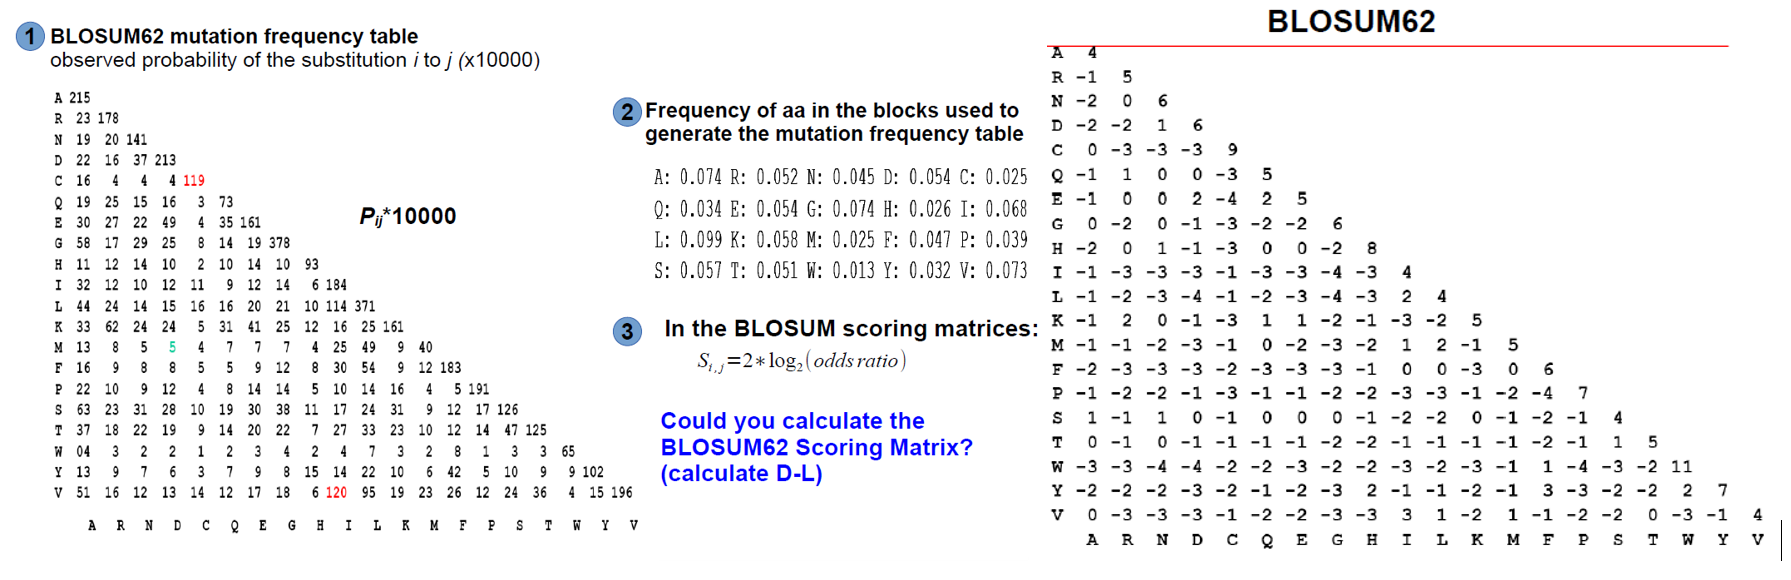
\includegraphics[width = \textwidth]{figs/ejercicio-blosum.png}
\end{figure}

\subsection{Exercise 12}
We performed a BLAST search using a human protein (X) as query against all \textit{Caenorhabditis elegans} proteins and got several hits. The figure below shows two of them.

\begin{figure}[htbp]
\centering
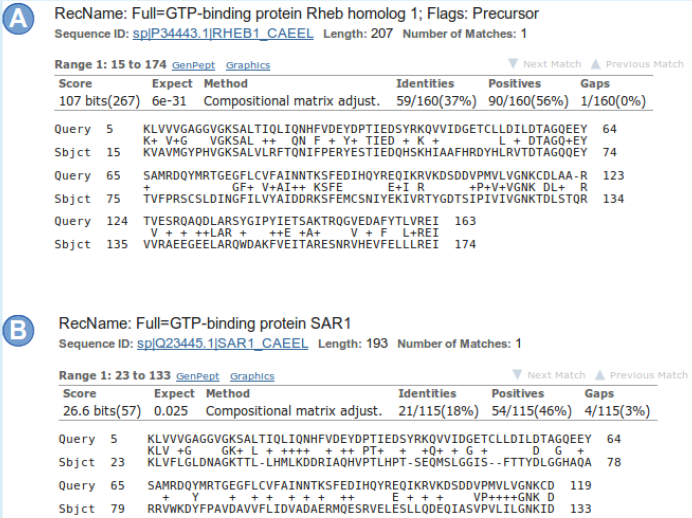
\includegraphics[width = 0.5\textwidth]{figs/exam-ex12.png}
\end{figure}

Indicate which of the following statements are correct:
\begin{enumerate}
\item Protein X and B share less than 25\% identity: \textbf{True, 18\%}
\item Protein X and A share a 37\% homology: \textbf{False, they are homologs, but this cannot be calculated on percentage; 37\% is the identity, not homology.}
\item Protein X and A are very likely to be homologs: \textbf{True, from 30\% identity onwards it can be considered as homology.}
\item Protein X and B are likely to have similar function/structure: \textbf{False}
\end{enumerate}

\subsection{Exercise 13}
Indicate which algorithm is best suited to solve the following alignments:
\begin{enumerate}
\item Alignment of two proteins that I suspect only share a short domain (I need to get the actual alignment): \textbf{Smith-Waterman's local alignment}.
\item A simple way to explore if a sequence contains duplicated regions: \textbf{Dot-matrix}
\item I need the optimal (best possible) alignment between two sequences: \textbf{Needleman-Wunsch's global alignment with dynamic programming}
\item Compare a protein sequence agains a large database in a short time: \textbf{word-based heuristic algorithm like BLAST}
\end{enumerate}

\subsection{Exercise 14}
What is the minimum number of permutations (minimum number of score values from random alignments) that we would need to determine if a given score has an associated p-value of <0.001? \textbf{ 1000 permutations, since 0.001 = 1/1000}

\subsection{Exercise 16}
What is the uncertainty (in bits) about the nucleotide residue occupying at a given DNA position? \textbf{2}. 
\begin{figure}[htbp]
\centering
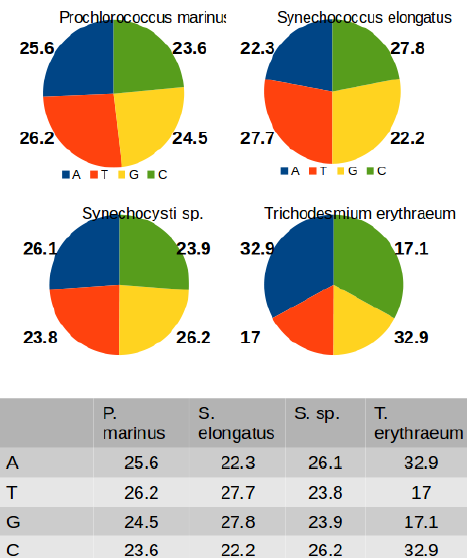
\includegraphics[width = 0.3\textwidth]{figs/exam-ex16.png}
\end{figure}
What is the entropy for a random position in the cyanobacteria genomes depicted in the figure?
\begin{itemize}
\item P. marinus: $-(0.256 \cdot log_2 (0.256) + 0.236 \cdot log_2(0.236) + 0.262 \cdot log_2 (0.262) + 0.245 \cdot log_2(0.245)) =  1.998 $
\item S. elongatus: $-(0.223 \cdot log_2 (0.223) + 0.278 \cdot log_2(0.278) + 0.277 \cdot log_2 (0.277) + 0.222 \cdot log_2(0.222)) =  1.991 $
\item S. sp.: $-(0.261 \cdot log_2 (0.261) + 0.239 \cdot log_2(0.239) + 0.238 \cdot log_2 (0.238) + 0.262 \cdot log_2(0.262)) =  1.998 $
\item T. erythraeum: $-(0.329 \cdot log_2 (0.329) + 0.171 \cdot log_2(0.171) + 0.17 \cdot log_2 (0.17) + 0.329 \cdot log_2(0.329)) =  1.926 $
\end{itemize}

What is the maximum possible entropy for a position in a DNA molecule? \textbf{2}. With this in mind, how much information does the human genome hold (in bits)? $2 \cdot 3 \cdot 10^9 = 6,000,000,000$ and in MBytes? $6,000,000,000 / 8 = 750,000,000 bytes / 10^6 = 750 MBytes$

What is the maximum theoretical entropy for a position in a protein sequence (in bits)?  $- \sum_{1}^{20} (\frac{1}{20} \cdot log_2(\frac{1}{20})) = 4.322$

\subsection{Exercise 27}
Determine the average length of the restriction fragments produced by the six-cutter restriction enzyme Smal that cuts the restriction site CCCGGG. Consider the case of (a) a genome with C+G content of 70\% and (b) a genome with G+C content of 30\%. In both cases, assume that the genomic sequence can be represented by a multinomial model with probabilities of nucleotides such that pG = pC and pA = pT. 

What would be the average length of the restriction fragments in case (a)? 
C and G have in total 70\% probability, so each has 35\%. The probability of the fragment in the human genome would be $0.35^6 \cdot 3 \cdot 10^9 = 5514796.875$. This represents the number of times the restriction enzyme would cut. To get the length of each piece: $3 \cdot 10^9 / 5514796.875 = 543.99 \approx 544$

What would be the average length of the restriction fragments in case (b)? 
C and G have in total 30\% probability, so each has 15\%. The probability of the fragment in the human genome would be $0.15^6 \cdot 3 \cdot 10^9 = 34171.875$. This represents the number of times the restriction enzyme would cut. To get the length of each piece: $3 \cdot 10^9 / 34171.875 = 87791.495 \approx 87791$

\subsection{Exercise 29}
A 4200nt long DNA fragment from the genome of bacteria \textit{Bioquimicus sp.} was sequenced and the results used to estimate the parameters of a Markov Chain model representation of this DNA. The observed counts for the sixteen possible dinucleotides in the + strand are shown in the table below, where rows indicate the first nucleotide and columns the second nucleotide of the dinucleotide.

\begin{table}[htbp]
\centering
\begin{tabular}{l | l l l l }
& A & C & G & T \\ \hline
A & 510 & 380 & 210 & 190 \\
C & 240 & 170 & 360 & 230 \\
G & 370 & 200 & 220 & 210 \\
T & 190 & 170 & 220 & 220
\end{tabular}
\end{table}

Find the maximum likelihood estimates of the transition probabilities $P_{TT}$ and $P_{AG}$ of the Markov chain model of the positive strand of this DNA:
$$P_{TT+} = \frac{220}{220+220+170+190} = 0.275$$
$$P_{AG+} = \frac{210}{210+190+380+510} = 0.163$$

Find also the transition probabilities $P_{TT}$ and $P_{AG}$ of the Markov chain model of the negative strand of this DNA:
$$P_{TT-} = \frac{AA}{AA + CA + GA + TA} = \frac{510}{510+240+370+190} = 0.389$$
$$P_{AG-} = \frac{CT}{CT + AT + GT + TT} = \frac{230}{230+190+210+220} = 0.271$$

\subsection{Exercise 30}
Life has just been discovered in Mars. Interestingly, martian microbes have proteins composed only by three aminoacids (X, Y, Z). Scientists have been able to generate some alignments from related martian proteins and from them calculated the mutation frequency table shown below (P*60). To calculate the entries of the martian scoring matrix, use the formula $S_{i,j} = 2 \cdot log_2(odds ratio)$

\begin{table}[htbp]
\centering
\begin{tabular}{l l l l || l }
& X & Y & Z & freq \\ \hline
X & 28 &  &  & 0.58333 \\
Y & 8 & 6 &  & 0.25 \\
Z & 6 & 10 & 2 & 0.1666 \\
\end{tabular}
\end{table}

What would be the value for the entry for the X to Z substitution in the corresponding scoring matrix?
$$2 \cdot log_2(\frac{6/60}{0.58333 \cdot 0.1666}) = 0.082 \approx 0$$

What would be the value for the entry for the Y to Y substitution in the corresponding scoring matrix?
$$2 \cdot log_2(\frac{6/60}{0.25 \cdot 0.25}) = 1.356 \approx 1$$

If all the entries in the mutation table were the same (e.g. all of them were 10 corresponding to a mutation of 10/60), the entries in the scoring matrix would be the same: \textbf{False, since the amino acid mutation is different.}

\subsection{Exercise 204}
The logo MA0598 below represents the binding sites for the transcription factor EHF. How many EHF binding sites would you expect in the human genome assuming a multinomial model with equal frequencies for all four nucleotides?

\begin{figure}[htbp]
\centering
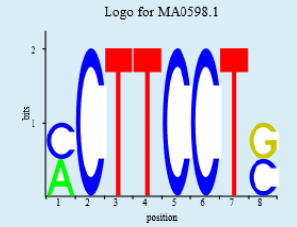
\includegraphics[width = 0.3\textwidth]{figs/exam-ex204.png}
\end{figure}

$$0.25^6 \cdot 0.5^2 \cdot 3 \cdot 10^9 = 183105.4688$$

\subsection{Exercise 203}
The sequence logo shown below was derived from the alignmed of 31 binding sites for the transcription factor XX. The matrix below the logo contains the number of nucleotides found at each position, but the columns have been shuffled so that the columns of the matrix (c1 to c6) do not necessarily correspond to each position in the logo (position 1 - 6). In addition, we do not know which nucleotide is recorded in each row of the matrix. Reconstruct the original order of columns in the matrix by matching the following terms:

\begin{figure}[htbp]
\centering
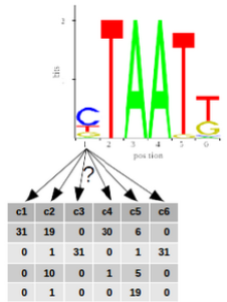
\includegraphics[width = 0.3\textwidth]{figs/exam-ex203.png}
\end{figure}

Positions 3 and 4 of the logo are the same, so we can conclude that they correspond to columns c3 and c6 of the matrix. Since these positions only have A, row 2 of the matrix has to represent A. Position 2 of the logo only has a T, which means that it must be column c1 and that row 1 is T. Position 1 of the logo contains all nucleotides, meaning that it can be either c2 or c5. However, the most frequent nucleotide is C, and since we know that row 1 is T, column c2 is excluded and c5 left (and row 4 must be C).

\begin{itemize}
\item Position 3 of the logo: \textbf{Column c6}
\item Position 1 of the logo: \textbf{Column c5}
\item Position 6 of the logo: \textbf{Column c2}
\item Row 2 of the matrix: \textbf{Counts for A}
\item Row 1 of the matrix: \textbf{Counts for T}
\end{itemize}

\end{document}
